% Options for packages loaded elsewhere
\PassOptionsToPackage{unicode}{hyperref}
\PassOptionsToPackage{hyphens}{url}
\PassOptionsToPackage{space}{xeCJK}
%
\documentclass[
  11pt,
  a4paper,
]{ctexart}
\usepackage{amsmath,amssymb}
\usepackage{lmodern}
\usepackage{setspace}
\usepackage{iftex}
\ifPDFTeX
  \usepackage[T1]{fontenc}
  \usepackage[utf8]{inputenc}
  \usepackage{textcomp} % provide euro and other symbols
\else % if luatex or xetex
  \usepackage{unicode-math}
  \defaultfontfeatures{Scale=MatchLowercase}
  \defaultfontfeatures[\rmfamily]{Ligatures=TeX,Scale=1}
  \setmainfont[]{Noto Serif CJK SC}
  \ifXeTeX
    \usepackage{xeCJK}
    \setCJKmainfont[]{Noto Serif CJK SC}
  \fi
  \ifLuaTeX
    \usepackage[]{luatexja-fontspec}
    \setmainjfont[]{Noto Serif CJK SC}
  \fi
\fi
% Use upquote if available, for straight quotes in verbatim environments
\IfFileExists{upquote.sty}{\usepackage{upquote}}{}
\IfFileExists{microtype.sty}{% use microtype if available
  \usepackage[]{microtype}
  \UseMicrotypeSet[protrusion]{basicmath} % disable protrusion for tt fonts
}{}
\makeatletter
\@ifundefined{KOMAClassName}{% if non-KOMA class
  \IfFileExists{parskip.sty}{%
    \usepackage{parskip}
  }{% else
    \setlength{\parindent}{0pt}
    \setlength{\parskip}{6pt plus 2pt minus 1pt}}
}{% if KOMA class
  \KOMAoptions{parskip=half}}
\makeatother
\usepackage{xcolor}
\IfFileExists{xurl.sty}{\usepackage{xurl}}{} % add URL line breaks if available
\IfFileExists{bookmark.sty}{\usepackage{bookmark}}{\usepackage{hyperref}}
\hypersetup{
  pdftitle={温县耕地土壤侵蚀与土壤健康研究},
  pdfauthor={EnvMatch-SEH 项目},
  hidelinks,
  pdfcreator={LaTeX via pandoc}}
\urlstyle{same} % disable monospaced font for URLs
\usepackage[margin=2cm]{geometry}
\usepackage{longtable,booktabs,array}
\usepackage{calc} % for calculating minipage widths
% Correct order of tables after \paragraph or \subparagraph
\usepackage{etoolbox}
\makeatletter
\patchcmd\longtable{\par}{\if@noskipsec\mbox{}\fi\par}{}{}
\makeatother
% Allow footnotes in longtable head/foot
\IfFileExists{footnotehyper.sty}{\usepackage{footnotehyper}}{\usepackage{footnote}}
\makesavenoteenv{longtable}
\usepackage{graphicx}
\makeatletter
\def\maxwidth{\ifdim\Gin@nat@width>\linewidth\linewidth\else\Gin@nat@width\fi}
\def\maxheight{\ifdim\Gin@nat@height>\textheight\textheight\else\Gin@nat@height\fi}
\makeatother
% Scale images if necessary, so that they will not overflow the page
% margins by default, and it is still possible to overwrite the defaults
% using explicit options in \includegraphics[width, height, ...]{}
\setkeys{Gin}{width=\maxwidth,height=\maxheight,keepaspectratio}
% Set default figure placement to htbp
\makeatletter
\def\fps@figure{htbp}
\makeatother
\setlength{\emergencystretch}{3em} % prevent overfull lines
\providecommand{\tightlist}{%
  \setlength{\itemsep}{0pt}\setlength{\parskip}{0pt}}
\setcounter{secnumdepth}{-\maxdimen} % remove section numbering
\usepackage{fancyhdr}
\usepackage{etoolbox}
\setlength{\headheight}{15pt}
\pagestyle{fancy}
\fancyhf{}
\fancyhead[L]{温县耕地土壤侵蚀与土壤健康研究}
\fancyfoot[C]{\thepage}
\let\origmaketitle\maketitle
\renewcommand{\maketitle}{\origmaketitle\thispagestyle{empty}\clearpage}
\apptocmd{\tableofcontents}{\clearpage}{}{}
\ifLuaTeX
  \usepackage{selnolig}  % disable illegal ligatures
\fi

\title{温县耕地土壤侵蚀与土壤健康研究}
\usepackage{etoolbox}
\makeatletter
\providecommand{\subtitle}[1]{% add subtitle to \maketitle
  \apptocmd{\@title}{\par {\large #1 \par}}{}{}
}
\makeatother
\subtitle{从数据准备到空间分析的完整故事}
\author{EnvMatch-SEH 项目}
\date{2026年11月4日}

\begin{document}
\maketitle

{
\setcounter{tocdepth}{1}
\tableofcontents
}
\setstretch{1.15}
\textbf{阅读说明：}

这份报告把项目从建立研究规则、检查数据、比较侵蚀和土壤健康，到分析空间差异、绘图和总结限制，连成一条故事线。读者不需要先懂统计学。遇到专业词时，报告会先用日常语言解释它，再说明它在本项目里做了什么。

报告讲的是项目已有记录所覆盖的工作，主要从2026年10月下旬开始。最初的野外采样、随机森林制图和侵蚀模型建模资料没有完整纳入本项目记录，因此不会把它们当作本项目重新做过的工作。研究区是河南省焦作市温县耕地。

\hypertarget{ux6458ux8981ux8fd9ux9879ux7814ux7a76ux505aux4e86ux4ec0ux4e48}{%
\section{摘要：这项研究做了什么？}\label{ux6458ux8981ux8fd9ux9879ux7814ux7a76ux505aux4e86ux4ec0ux4e48}}

项目想知道：在温县耕地里，土壤侵蚀较高的地方，土壤健康图上的数值是否往往较低？如果把环境条件相近的地方放在一起比较，这种关系还在不在？不同土壤指标的变化是不是一样？这种关系会不会随地点改变？

项目先把来源不同、大小不同、位置没有完全对齐的栅格图放到同一张30米网格上，再检查缺失值、零值、范围和土壤类型。随后，研究人员先比较全县的整体关系，再尝试把环境相近、侵蚀水平不同的地点配成对；之后又比较多种曲线、土壤类型和空间模型，并画出局部关系图和路径图。

目前最稳定的整体线索是：Aa\_20yr
越高，土壤含水量（SW）、土壤健康指数（SHI）和有机质（OM）的预测值通常越低。三者的
Spearman 秩相关分别为 -0.584、-0.469 和
-0.415。它们是地图像元之间的空间关联，不是几十万个独立实测样点，也不能单独证明侵蚀造成了健康下降。环境匹配后的配对差值仍呈负向，但数值更弱；局部空间模型也显示不同地方的关系大小不完全一样。

要特别记住：Phase F 到 Phase J 的大量结果属于用户授权的探索性 Oracle
分析。它们允许按健康结果寻找更有利的分组或模型，所以适合发现线索和提出下一步问题，不等于预先锁定方案后的正式验证。正式研究的环境和匹配阶段仍有未解决的数据来源、时间单位和设计锁定问题；既有
PCNM 结果也还没有可用的结果表来做比较。

\begin{quote}
\textbf{一句话主线：}
先让地图格子能够公平对照，再问``总体上是否相关''，然后问``环境相近时是否还相关''，最后看``这种关系在哪里更强、不同健康指标是否不同''，同时不断检查数据和模型有没有把地图纹理误当成独立证据。
\end{quote}

\hypertarget{ux4e00ux4e3aux4ec0ux4e48ux8981ux505aux8fd9ux9879ux7814ux7a76}{%
\section{一、为什么要做这项研究？}\label{ux4e00ux4e3aux4ec0ux4e48ux8981ux505aux8fd9ux9879ux7814ux7a76}}

土壤侵蚀可以理解为土壤被水或其他过程带走。耕地土壤健康则不是一个单独的量尺：它包含土壤里有机质、养分、水分、酸碱度、微生物等不同方面。一个地方同时有较高侵蚀和较低健康预测值，可能是因为侵蚀，也可能是因为坡度、地形湿度、气候、土类、耕作方式或制图误差等因素共同变化。

所以项目不只问``这两张地图是不是一高一低''，还要问：如果只比较环境条件相近的地点，关系是否还存在？换到不同土壤或地形环境，关系是否改变？九项健康结果是否都朝同一方向变化？空间上的近邻是否让看起来很大的样本数显得比实际证据更强？

研究总纲把这些问题分成五个科学问题：环境相似时是否仍有关联、关系是否因环境而异、不同类型的健康指标是否不同、与既有
PCNM
空间控制结果是否一致，以及怎样改进环境匹配和推断质量。研究总纲规定研究方向；项目执行规则和阶段门说明什么时候可以进入下一步。\href{RESEARCH_CHARTER.md}{研究总纲}；\href{governance/RESEARCH_STAGE_GATES.md}{阶段门规则}

本项目使用已经算好的实际侵蚀栅格 Aa，不重建或验证 RUSLE 因子乘积。RUSLE
是一种估算土壤侵蚀的计算框架；本轮工作按项目指令直接使用已有 Aa
输入。项目也没有重新采集野外土壤样品。已有土壤健康和八项指标图层是随机森林预测栅格：随机森林可以粗略理解为许多决策树一起投票的预测方法。

\hypertarget{ux4e8cux5148ux628aux5730ux56feux4e0aux7684ux4e00ux683cux8bf4ux6e05ux695a}{%
\section{二、先把``地图上的一格''说清楚}\label{ux4e8cux5148ux628aux5730ux56feux4e0aux7684ux4e00ux683cux8bf4ux6e05ux695a}}

\hypertarget{ux7c73ux50cfux5143ux662fux4ec0ux4e48}{%
\subsection{2.1
30米像元是什么？}\label{ux7c73ux50cfux5143ux662fux4ec0ux4e48}}

栅格图可以想成一张由小方格组成的棋盘。这里的基本格子宽30米、长30米，面积是900平方米。每个格子存一个侵蚀值、土壤健康值或环境值。

一格不是一位农民、一块田，也不是一次独立的现场测量。邻近格子往往共享土壤、地形和制图信息，数值彼此相似。因此``有几十万个格子''不等于``做了几十万个互相独立的实验''。报告里的像元数只说明地图覆盖了多少格，不能直接当成独立实测样本量。

\hypertarget{ux4e24ux671fux4fb5ux8680ux56fe}{%
\subsection{2.2 两期侵蚀图}\label{ux4e24ux671fux4fb5ux8680ux56fe}}

\begin{itemize}
\tightlist
\item
  \textbf{Aa\_20yr}：项目沿用的20年平均实际侵蚀图。
\item
  \textbf{Aa\_2020}：项目沿用的2020年实际侵蚀图。
\item
  \textbf{实际侵蚀 Aa}：这里使用已经提供的侵蚀估算结果。Aa
  的单位和准确的20年起止范围没有从栅格元数据中核实，所以本报告只比较其相对大小，不把未确认的单位写成吨/公顷/年等具体物理单位。
\item
  \textbf{log1p(Aa)}：先对侵蚀值加1再取对数。这样高值不会把低值挤到图的一小角，零值也能保留。它是建模时的刻度转换，不是把侵蚀``变成零''。
\end{itemize}

\hypertarget{ux4e5dux9879ux5065ux5eb7ux7ed3ux679c}{%
\subsection{2.3
九项健康结果}\label{ux4e5dux9879ux5065ux5eb7ux7ed3ux679c}}

项目分析一个综合结果和八项土壤指标：

\begin{longtable}[]{@{}lll@{}}
\toprule
缩写 & 通俗名称 & 可以怎样理解 \\
\midrule
\endhead
SHI & 土壤健康指数 & 把多项指标合成的总体分数；本项目沿用既有预测图 \\
AN & 碱解氮 & 一种与土壤可供养分有关的指标 \\
OM & 有机质 & 土壤中动植物残体分解形成的有机物 \\
CEC & 阳离子交换量 & 粗略反映土壤留住、交换部分养分离子的能力 \\
pH & 酸碱度 & 表示土壤偏酸还是偏碱 \\
SW & 土壤含水量 & 土壤中水分的多少 \\
BD & 土壤容重 & 一定体积土壤有多紧实，可帮助理解孔隙和压实程度 \\
MBC & 微生物量碳 & 土壤微生物体量的一种指标 \\
RESP & 土壤呼吸 & 土壤生物活动释放气体的一种观测或预测指标 \\
\bottomrule
\end{longtable}

这些指标的``高''不一定都代表``更健康''。例如，pH 不是越高越好，RESP
也不能只凭高低判定健康。因此报告多数时候描述``指标数值和侵蚀的关系''，不会擅自把每项都改造成统一的健康分数。

项目把 SW、BD 放在物理维度，把 OM、AN、CEC、pH 放在化学维度，把
MBC、RESP
放在生物维度。这是帮助读者整理指标的分类，不等于已经用可靠载荷和权重验证了三个潜在因子。

\hypertarget{ux4e09ux9879ux76eeux9075ux5b88ux7684ux4e24ux79cdux5206ux6790ux89c4ux5219}{%
\section{三、项目遵守的两种分析规则}\label{ux4e09ux9879ux76eeux9075ux5b88ux7684ux4e24ux79cdux5206ux6790ux89c4ux5219}}

项目把研究分为正式实证模式和探索性 Oracle 模式。

\hypertarget{ux6b63ux5f0fux6a21ux5f0fux5148ux5b9aux6bd4ux8f83ux529eux6cd5ux518dux770bux5065ux5eb7ux7ed3ux679c}{%
\subsection{正式模式：先定比较办法，再看健康结果}\label{ux6b63ux5f0fux6a21ux5f0fux5148ux5b9aux6bd4ux8f83ux529eux6cd5ux518dux770bux5065ux5eb7ux7ed3ux679c}}

正式研究要求先根据环境资料决定使用哪些变量、怎样分组、怎样配对；不能先看
SHI
或八项指标，再挑最容易出现预期关系的方案。这样做是为了避免``先看答案再挑题目''。

\hypertarget{oracle-ux63a2ux7d22ux83b7ux51c6ux8bd5ux4e0dux540cux529eux6cd5ux4f46ux8981ux628aux9009ux62e9ux8fc7ux7a0bux8bb2ux51faux6765}{%
\subsection{Oracle
探索：获准试不同办法，但要把选择过程讲出来}\label{oracle-ux63a2ux7d22ux83b7ux51c6ux8bd5ux4e0dux540cux529eux6cd5ux4f46ux8981ux628aux9009ux62e9ux8fc7ux7a0bux8bb2ux51faux6765}}

用户授权后，项目另开 Oracle
探索模式。它可以试不同分组、匹配距离、模型和样本子集，观察哪些地方值得继续研究。它必须单独保存，并写明结果导向筛选；筛选出的漂亮结果不能冒充独立验证或正式因果证据。

这里有一个容易混淆的命名：正式流程的 G0-G5 是``阶段门''；Phase
F、G、H、I、J 是后来 Oracle
运行的阶段名字。它们字母有重叠，但不是同一套阶段，也就是说``Phase F
做过分析''不代表正式 G4 或 G5 已经通过。

\hypertarget{ux56dbux4eceux6570ux636eux8fdbux6765ux5230ux53efux4ee5ux6bd4ux8f83ux9879ux76eeux600eux6837ux4e00ux6b65ux6b65ux94faux8def}{%
\section{四、从数据进来，到可以比较：项目怎样一步步铺路}\label{ux56dbux4eceux6570ux636eux8fdbux6765ux5230ux53efux4ee5ux6bd4ux8f83ux9879ux76eeux600eux6837ux4e00ux6b65ux6b65ux94faux8def}}

\hypertarget{ux7b2cux4e00ux6b65ux5efaux7acbux89c4ux5219ux548cux53efux91cdux590dux7684ux5de5ux4f5cux6d41ux7a0b}{%
\subsection{第一步：建立规则和可重复的工作流程}\label{ux7b2cux4e00ux6b65ux5efaux7acbux89c4ux5219ux548cux53efux91cdux590dux7684ux5de5ux4f5cux6d41ux7a0b}}

项目先把研究总纲、数据规则、方法、工作流程和审查要求写清楚，并建立
Python 命令行流程。流程可按``检查数据 → 建立统一数据库 → 检查环境变量 →
分组 → 检查侵蚀差异 → 配对 → 分析健康结果 → 对照 PCNM →
生成报告''依次运行。

为什么要这样做？因为同一套数据若被人用不同参数重复处理，很容易得到无法解释的差别。每次运行应留下输入、配置、软件版本和结果目录，方便回头核对。

最初版本用合成数据做了44项软件检查并通过。这说明流程在这些测试输入上能按预期工作；合成数据不是温县实测，也不证明科学结论正确。

\hypertarget{ux7b2cux4e8cux6b65ux76d8ux70b9ux6587ux4ef6ux68c0ux67e5ux6805ux683cux7f51ux683c}{%
\subsection{第二步：盘点文件、检查栅格网格}\label{ux7b2cux4e8cux6b65ux76d8ux70b9ux6587ux4ef6ux68c0ux67e5ux6805ux683cux7f51ux683c}}

首轮数据清点登记了312个来源文件，读取了77组栅格数据。9组、32个文件条目属于内容重复或配套元数据文件。两个矢量数据缺少部分索引、属性或投影配套文件，不能完整用来独立确认研究区边界。

为什么网格对齐很重要？把两张透明方格纸叠在一起，如果小格的位置差半格，同一个数组位置可能落在两块不同田地上。那样算出来的``相关''可能只是错位造成的。

项目使用一张统一的耕地掩膜作为参考网格。候选掩膜有1240行、977列、30米分辨率、EPSG:32649坐标系，共392,527个有效像元；按每格900平方米换算，约353.274平方公里。研究总纲里已有面积约347.877平方公里，两者相差约5.397平方公里（约1.55\%）。由于边界文件缺少配套文件，无法在本轮独立判定差别来自边界版本还是栅格掩膜，因此保留差异，没有硬把面积改成某一个数字。

侵蚀、环境和健康栅格原来有不同的行列数、像元位置或坐标信息。项目将连续量对齐到模板：主要侵蚀输入用面积平均方式汇总到统一格网，并保留最近邻方式作为敏感性比较；连续环境和健康图用双线性插值；土壤类型这类类别图用最近邻，避免把``土类26和27''插成小数类别。

对齐之后，主要数据库记录了392,527个耕地像元。部分分析还要求变量同时有值，所以每个分析的有效样本数不同。早期两期侵蚀共同有效像元为387,596；后续当前
CEC 有效像元为387,448；Phase J
核心环境完整样本为293,145。这些数字对应不同变量条件，不能互相替代。

\hypertarget{ux7b2cux4e09ux6b65ux5148ux68c0ux67e5ux4fb5ux8680ux66b4ux9732ux548cux73afux5883ux518dux8003ux8651ux5339ux914d}{%
\subsection{第三步：先检查侵蚀暴露和环境，再考虑匹配}\label{ux7b2cux4e09ux6b65ux5148ux68c0ux67e5ux4fb5ux8680ux66b4ux9732ux548cux73afux5883ux518dux8003ux8651ux5339ux914d}}

正式方案优先考虑高程、曲率、地形湿度指数 TWI、地表温度 LST 等非 RUSLE
直接因子，土壤类型用于分层。TWI
可以理解为地形上某处较容易汇集水分的相对程度。主匹配距离不放入
R、K、LS、C、P，因为这些直接参与了侵蚀计算；否则比较环境时可能把侵蚀公式本身的信息又加回去。

正式方案要求保留零侵蚀格子，用 log1p(Aa)
表示暴露，并核查组内侵蚀是否有足够差异。如果某组内所有点侵蚀都差不多，就无法比较``高侵蚀''和``低侵蚀''。

分组试验的质量并不理想：部分聚类的轮廓系数约在 -0.0147 到 0.0019
之间，接近零或小于零，表示组与组并没有清晰分开；不同参数结果的调整兰德指数约0.381-0.857，说明分组稳定性不一。500米、8组等探索配置可以找到不少配对，例如20年平均侵蚀一个候选有103,586对、2020年一个候选有114,399对，环境标准化差异最大值分别约0.0203和0.032。这说明``能配到点''不等于``正式设计已被证明合格''。这些只是可行性探索，没锁定正式参数。

\hypertarget{ux6b63ux5f0fux7814ux7a76ux9636ux6bb5ux95e8ux7684ux5f53ux524dux72b6ux6001}{%
\subsection{正式研究阶段门的当前状态}\label{ux6b63ux5f0fux7814ux7a76ux9636ux6bb5ux95e8ux7684ux5f53ux524dux72b6ux6001}}

\begin{longtable}[]{@{}
  >{\raggedright\arraybackslash}p{(\columnwidth - 4\tabcolsep) * \real{0.33}}
  >{\raggedright\arraybackslash}p{(\columnwidth - 4\tabcolsep) * \real{0.33}}
  >{\raggedright\arraybackslash}p{(\columnwidth - 4\tabcolsep) * \real{0.33}}@{}}
\toprule
阶段门 & 要回答的问题 & 项目目前能说到哪里 \\
\midrule
\endhead
G0 科研治理 & 研究方向、权限和审查规则清楚吗？ &
总纲、协议和阶段门文件已经建立 \\
G1 数据接入 & 找到了哪些文件，它们代表什么？ &
完成了文件清点和初步映射；有些变量解释仍是暂定 \\
G2 栅格与模型数据质量 &
数据位置、单位、时间、覆盖和缺失是否足以支持正式分析？ &
完成许多对齐和可读性检查；Aa
的物理单位和精确时间口径仍待来源证明，正式质量门未完整通过 \\
G3 环境变量 &
环境变量的意义、年份、缺失和与健康制图的共用信息是否充分核查？ &
有候选变量和分布检查；正式环境向量尚未完整锁定 \\
G4 匹配 & 环境是否平衡，组内侵蚀差异是否足够，规则是否不依赖健康结果？ &
Oracle 中做过多种匹配探索；正式匹配设计未锁定 \\
G5 健康响应与 PCNM 对照 & 正式设计下结果能否复现并与既有空间控制比较？ &
Oracle 有大量响应分析；正式 G5 未完成，PCNM
结果表缺失，因此不能给出一致性结论 \\
\bottomrule
\end{longtable}

阶段门不是``必须显著才算通过''。它要求数据和设计足以支持下一步，而不是要求结果符合预想。\href{governance/RESEARCH_STAGE_GATES.md}{阶段门规则}

\hypertarget{ux4e94ux83b7ux5f97ux6388ux6743ux540eux7684ux63a2ux7d22phase-f-ux5230-phase-j}{%
\section{五、获得授权后的探索：Phase F 到 Phase
J}\label{ux4e94ux83b7ux5f97ux6388ux6743ux540eux7684ux63a2ux7d22phase-f-ux5230-phase-j}}

下面这些阶段按时间顺序讲的是 Oracle
探索结果。每一步解决一个不同问题；样本数和模型并不都来自同一批像元。

\hypertarget{ux65e9ux671fux641cux7d22ux5b66ux4e60ux62dfux5408ux5f97ux597dux770bux4e0dux7b49ux4e8eux53efux9760}{%
\subsection{5.1
早期搜索：学习``拟合得好看''不等于可靠}\label{ux65e9ux671fux641cux7d22ux5b66ux4e60ux62dfux5408ux5f97ux597dux770bux4e0dux7b49ux4e8eux53efux9760}}

早期 Oracle
尝试登记了约4,030条探索记录、1,024次模型试验和2,448个子组结果。一次把样本缩到约5\%后的
SHI 模型，表观 R²
达到0.9977。R²可以粗略理解为``模型在眼前这些数据上跟着数值变化的程度''，高
R² 表示贴得很紧。

但在空间验证中，选定模型的验证表现曾为负 R²；Aa\_20yr 例子中验证 R²
约-0.069，而另一留出块的测试 R²
约0.470；2020年的对应值约-0.143和0.233。不同的验证块结果差别很大。负 R²
表示模型在那批未见过的地点上还不如简单地用平均值猜。

这一步的价值不是``找到了几乎完美的模型''，而是显示多次挑选后，眼前拟合可能被夸大。空间位置要整块留出，才更能检验模型能否用于新地方；而且所有挑选过程都应披露。

\hypertarget{phase-fux6bd4ux8f83ux51e0ux79cdux73afux5883ux5339ux914dux529eux6cd5}{%
\subsection{5.2 Phase
F：比较几种环境匹配办法}\label{phase-fux6bd4ux8f83ux51e0ux79cdux73afux5883ux5339ux914dux529eux6cd5}}

Phase F 比较直接回归、环境调整、土壤分组后配对、组内最近邻等方案。M3
是先按土壤类型和 K-means 分组的候选；M4
是在同一土壤类型内直接寻找环境和空间上接近、但侵蚀水平有差异的配对。K-means
是让电脑按变量相似程度自动分组的一种方法。

这一阶段用5公里空间块把研究区分成训练、验证和测试区域，并使用多个随机种子重复。这样做是为了避免把隔壁像元分别塞进训练集和测试集，让模型通过``记住邻居''显得很准。

在 M4 的20年侵蚀候选里，SHI、OM、SW 的平均高侵蚀端减低侵蚀端差值约为
-0.033、-2.854、-6.062；标准化配对斜率约 -0.123、-0.077、-0.204；表观 R²
约0.015、0.006、0.042。空间测试的 R²
多接近零，SW在一个候选中位数约0.040。数字显示方向大多为负，但配对差异并不强，预测到新空间块的能力有限。

这些结果是早期候选，不是最终唯一匹配版。Phase F 的 M4
环境距离卡尺为0.35，地理距离上限1000米，要求配对侵蚀百分位至少相差0.50。它与
Phase J 里另一套 M4/D4 设计不同，不能把所有 M4
样本简单拼在一起。\href{reviews/2026-10-26/PHASE_F_RESEARCH_REPORT.md}{Phase
F 报告}

\hypertarget{phase-gux770bux4e0dux540cux5206ux7ec4ux65b9ux5f0fux4f1aux4e0dux4f1aux6539ux53d8ux7b54ux6848}{%
\subsection{5.3 Phase
G：看不同分组方式会不会改变答案}\label{phase-gux770bux4e0dux540cux5206ux7ec4ux65b9ux5f0fux4f1aux4e0dux4f1aux6539ux53d8ux7b54ux6848}}

Phase G 比较土壤类型分组、K-means、Ward
层次聚类，以及按高程、TWI、地表温度、植被等环境变量分位分组。它关注``侵蚀与健康的关系在不同环境组里是否一样''。

全配对 M4 的20年侵蚀配对差值 Spearman 相关为 SHI -0.128、OM -0.114、SW
-0.192。Spearman
相关先把数值换成大小名次，再看两个名次是否一起增减；它适合描述单调关系，但不表示因果。

分组和响应方案经过 Oracle
搜索，所以某些组的结果比整体更明显，不能把``搜到最明显的组''说成预先预测成功。这一步说明土类、地形和分组算法可能改变估计，也让后续报告把每个总体分开。\href{reviews/2026-10-27/phase-g/PHASE_G_RESEARCH_REPORT.md}{Phase
G 报告}

\hypertarget{phase-hux68c0ux67e5ux96f6ux503cux4f4eux4fb5ux8680ux548cux5f2fux66f2ux5173ux7cfb}{%
\subsection{5.4 Phase
H：检查零值、低侵蚀和弯曲关系}\label{phase-hux68c0ux67e5ux96f6ux503cux4f4eux4fb5ux8680ux548cux5f2fux66f2ux5173ux7cfb}}

很多格子的侵蚀值为零。项目分别检查``有没有侵蚀''和``侵蚀大到什么程度''，并尝试线性、对数、二次曲线、分段曲线、自然样条、GAM、稳健回归、分位数回归和树模型。GAM
可以理解为让曲线自己弯，而不是强迫关系只能是一条直线。

两期 Aa 的经验分布曾给出候选断点：Aa\_20yr
约5.050，Aa\_2020约0.396692。但核密度图没有清楚的谷底，混合高斯模型也显示组间重叠、分类不确定。因此项目没有把断点当成自然法则或法定风险线，也没有把零侵蚀像元从主分析中删掉。断点只作敏感性比较。

为什么保留零值？如果删掉零值，研究对象就从``全部耕地''变成``有正侵蚀的耕地''。两种总体回答不同问题。Phase
H
同时保留全范围、零对正和两端都为正值的对照，并区分像元回归与配对差值回归。阶段共登记10,764条模型或子组记录，依旧是探索性搜索，不能把试过很多模型后最好的一个单独当作确认性结果。\href{reviews/2026-10-28/phase-h/PHASE_H_EXPLORATORY_REPORT.md}{Phase
H
探索报告}；\href{reviews/2026-10-29/phase-h/LOW_EROSION_REGIME_RESEARCH_REPORT.md}{低侵蚀专题}

\hypertarget{phase-iux4eceux603bux4f53ux5173ux7cfbux4e00ux8defux770bux5230ux5c40ux90e8ux5730ux56fe}{%
\subsection{5.5 Phase
I：从总体关系一路看到局部地图}\label{phase-iux4eceux603bux4f53ux5173ux7cfbux4e00ux8defux770bux5230ux5c40ux90e8ux5730ux56fe}}

Phase I 把探索拆成 I-1 到 I-8 和
I-C。I-2复用此前保存的匹配结果，I-3复用环境组结果，部分空间模型也复用已保存系数；不是每个编号都重新拟合了一套模型。更细的逐模块数据、模型和图件说明见\href{reviews/2026-10-31/phase-i/PHASE_I_FINAL_RESEARCH_REPORT.md}{Phase
I
综合报告}和\href{reviews/2026-10-31/phase-i/PHASE_I_CLOSURE_REPORT.md}{结题补充}。

\begin{longtable}[]{@{}
  >{\raggedright\arraybackslash}p{(\columnwidth - 6\tabcolsep) * \real{0.25}}
  >{\raggedright\arraybackslash}p{(\columnwidth - 6\tabcolsep) * \real{0.25}}
  >{\raggedright\arraybackslash}p{(\columnwidth - 6\tabcolsep) * \real{0.25}}
  >{\raggedright\arraybackslash}p{(\columnwidth - 6\tabcolsep) * \real{0.25}}@{}}
\toprule
模块 & 具体做了什么 & 为什么做 & 得到的主要信息 \\
\midrule
\endhead
I-1 全域关系 &
对九项健康结果分别算相关，检查零值与正值，比较空间块预测模型和 GAM 曲线
& 先建立``整张地图大致是什么样''的基线 & SW、SHI、OM
对20年侵蚀的负向秩相关最明显 \\
I-2 匹配关系 & 复用一套 M4 配对，分别看匹配端点和每对高低侵蚀端的差值 &
看环境近邻设计下关系是否仍在 & 配对差值仍多为负，但弱于全域像元关系 \\
I-3 环境差异 & 按土类、TWI、植被和地表温度等分组，比较组内斜率和交互 &
看关系会不会随环境背景改变 & 一些土类和湿度组负斜率较强；结果受 Oracle
搜索影响 \\
I-4 局部回归 & 在约240米空间单元上做 GWR 和局部共线性收缩模型 &
看同一条``平均线''是否遮住不同地区的变化 & SHI、OM、SW
的局部平均斜率为负，但不同模型幅度不同 \\
I-5 局部机器学习 & 比较局地随机森林、SHAP/ALE 解释和空间变化系数模型 &
检查非线性、局部预测和变量贡献图 &
局部随机划分容易让邻近位置重叠；空间测试中复杂曲面的增益很小 \\
I-6 局部空间聚集 & 计算邻域相关、双变量 LISA 和热点 &
区分``本格值低''和``周围一片呈同类格局'' &
能看到局部聚集，但热点数量依模型设置而变 \\
I-7 健康维度与既有成果 & 整理物理、化学、生物指标，并预留
PCNM/既有路径的对照栏 & 避免缺少源数据时凭印象补数 & PCNM 和旧 PLS-SEM
结果表没有找到，比较结论留空 \\
I-8 候选空间区 & 把高侵蚀、低 SHI 和局部负斜率组合成几个探索分区 &
形成后续现场核查线索 & 找到 T1 等候选区；阈值是 Oracle
分位点，不是法定边界 \\
I-C 标准 MGWR & 在同一空间均衡样本上比较标准 GWR 与 MGWR &
检查不同变量是否有不同的空间作用尺度 & Aa 对 SHI
的拟合带宽较局部；OM、SW 带宽接近搜索上限 \\
\bottomrule
\end{longtable}

\hypertarget{i-1ux4e5dux9879ux6307ux6807ux7684ux603bux4f53ux5173ux8054}{%
\subsubsection{I-1：九项指标的总体关联}\label{i-1ux4e5dux9879ux6307ux6807ux7684ux603bux4f53ux5173ux8054}}

在全掩膜像元中，Aa\_20yr 与九项健康结果的 Spearman
相关如下。这个表回答``数值总体上一起升还是一起降''，不是控制所有因素后的效果，也不是独立实测点的相关。

\begin{longtable}[]{@{}lrl@{}}
\toprule
健康结果 & Spearman ρ & 简单读法 \\
\midrule
\endhead
土壤含水量 SW & -0.584 & 九项中负向关系最明显 \\
土壤健康指数 SHI & -0.469 & 综合指数也有明显负向空间关系 \\
有机质 OM & -0.415 & 主要化学指标中负向关系较明显 \\
CEC & -0.286 & 解释必须考虑后文的公式耦合 \\
土壤呼吸 RESP & -0.272 & 中等偏弱负向排序关系 \\
碱解氮 AN & -0.233 & 较弱负向关系 \\
土壤容重 BD & -0.200 & 较弱负向关系 \\
微生物量碳 MBC & -0.118 & 较弱负向关系 \\
pH & -0.109 & 很弱负向关系 \\
\bottomrule
\end{longtable}

5公里空间块模型中，SHI、SW、OM 的标准化回归系数分别约为
-0.472、-0.595、-0.421；按空间块重抽样得到的区间也维持负向。不过很多结果的空间测试预测能力较小或为负，所以这些区间不能弥补数据来源、空间依赖和结果导向筛选的限制。

\begin{figure}
\centering
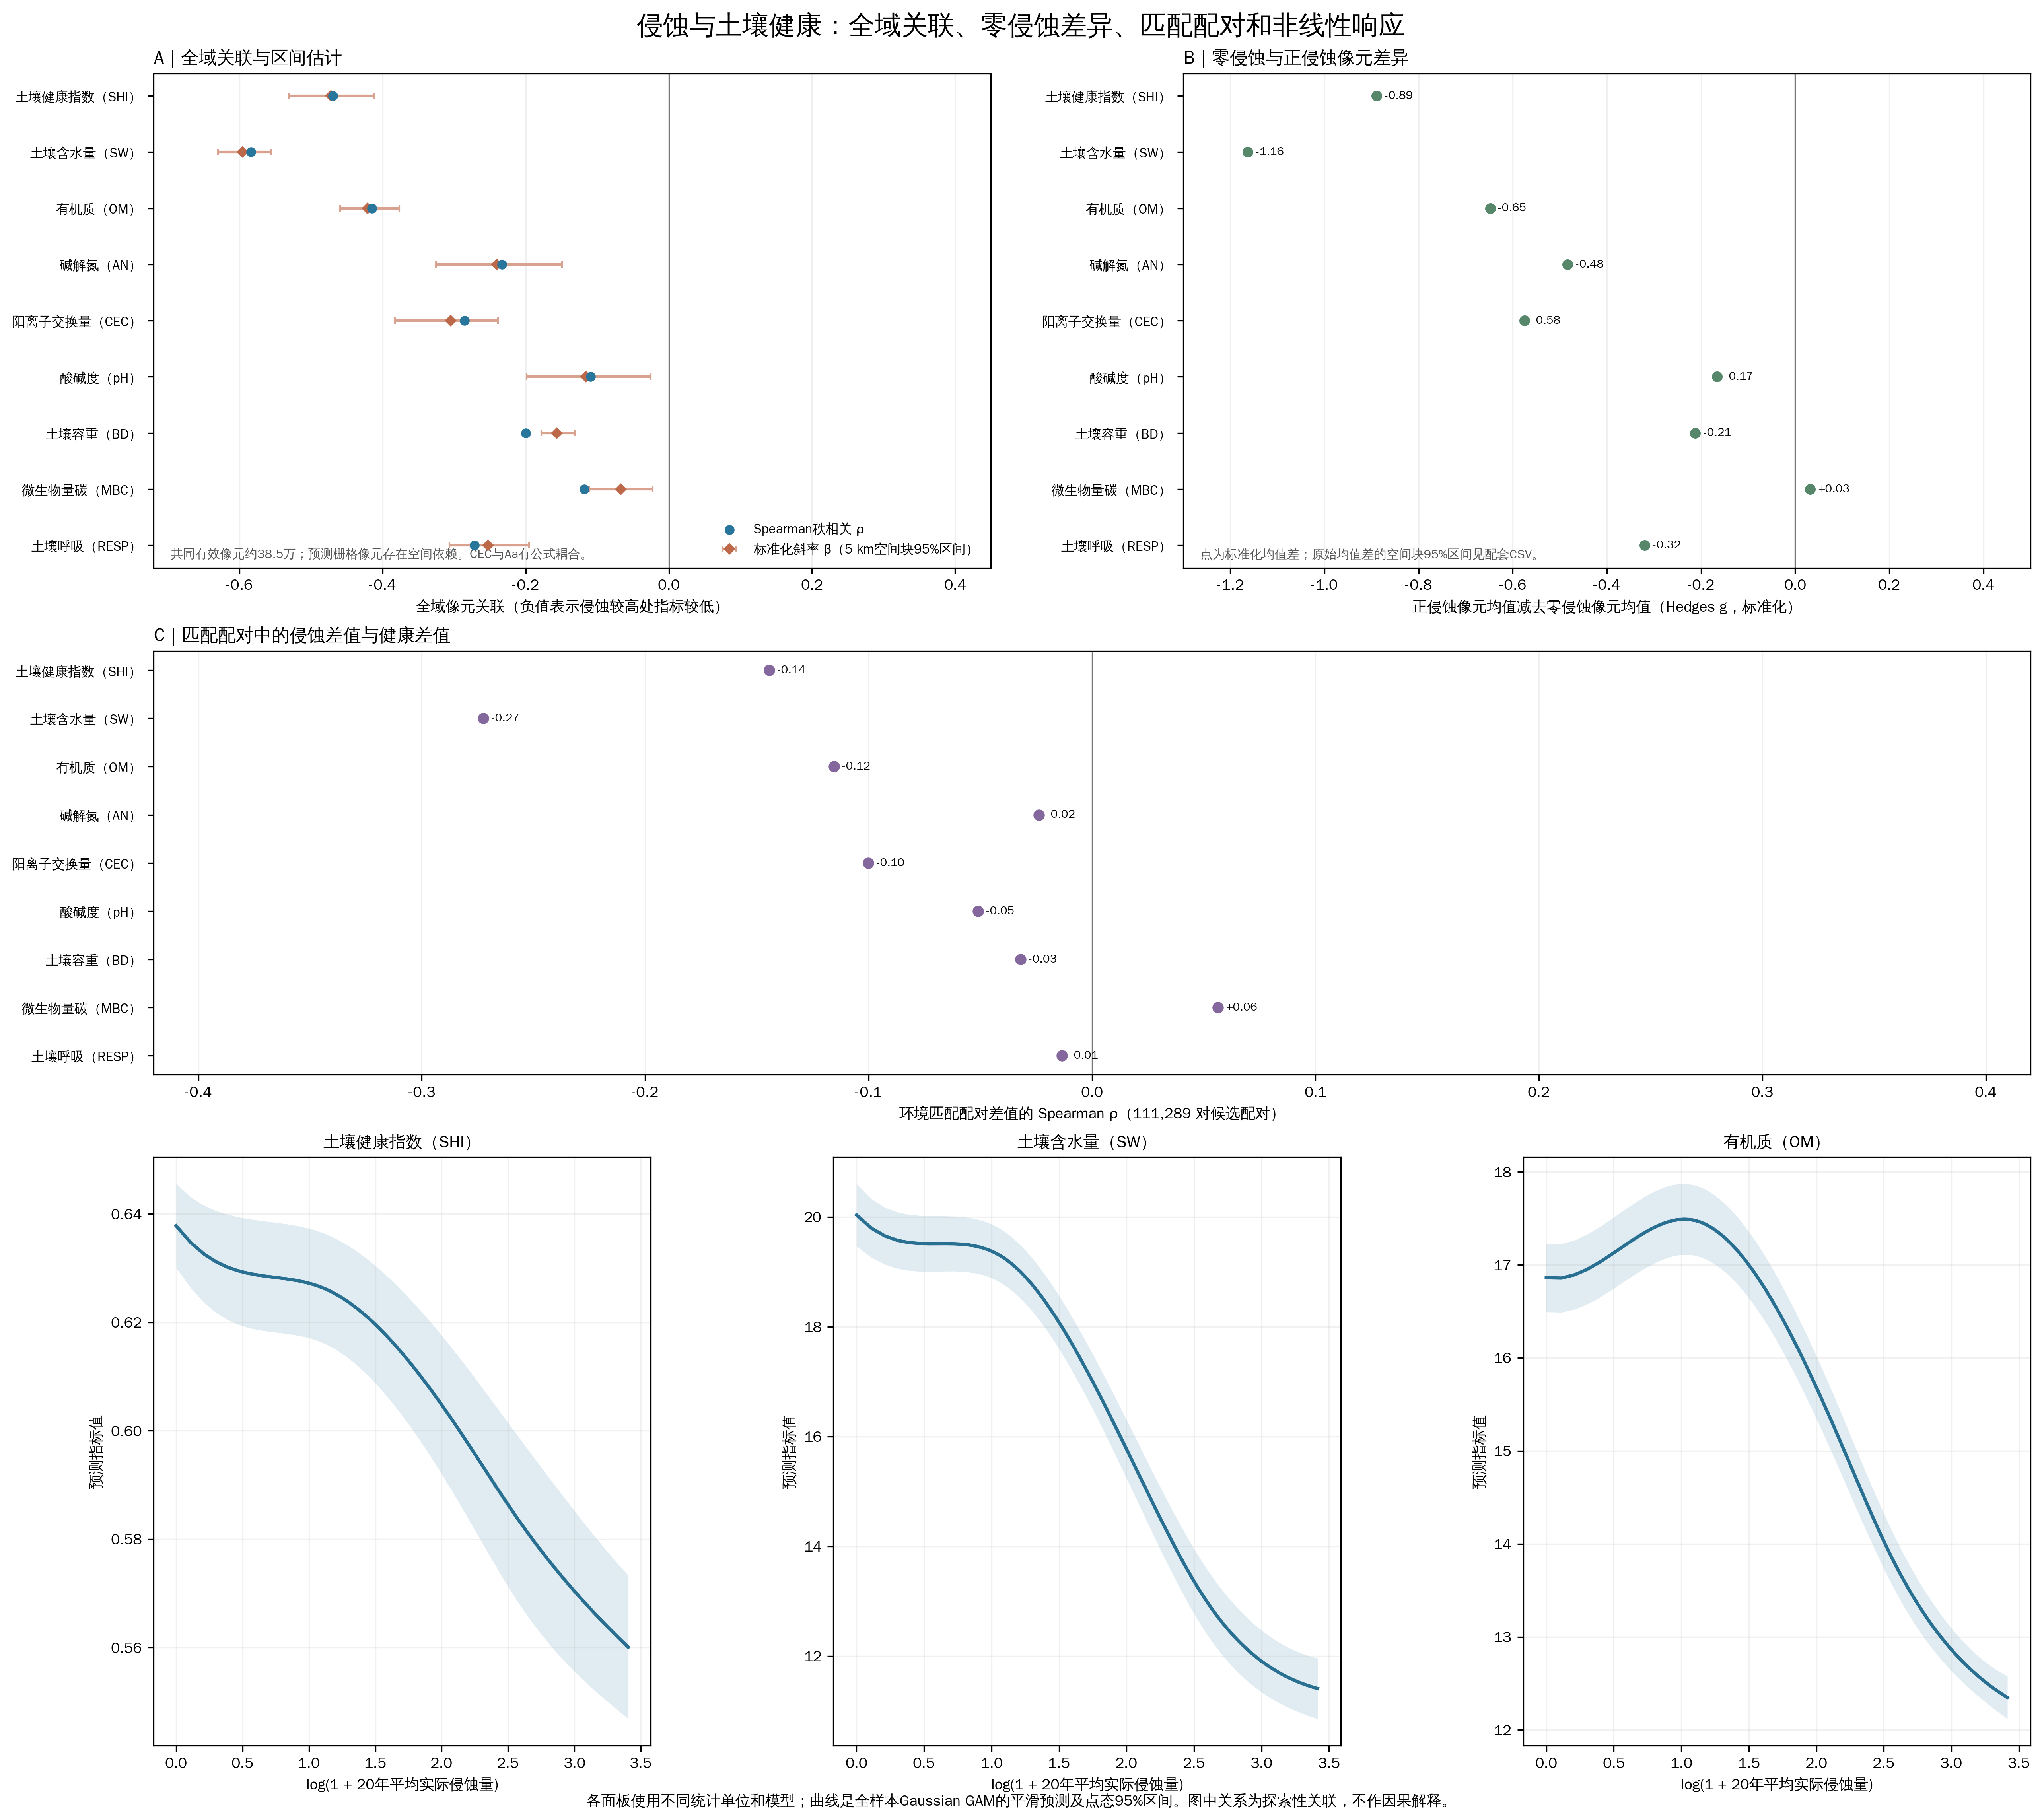
\includegraphics{reviews/2026-11-02/phase-j/figures/A_multimethod_erosion_health_response.png}
\caption{多方法综合图：上方依次比较全域关联、零侵蚀与正侵蚀差异、匹配配对差值；下方展示
SHI、SW、OM
的弯曲响应曲线。各面板样本和统计量不同，描述的是预测栅格关系，不是因果图。}
\end{figure}

\hypertarget{i-2ux5339ux914dux540eux5173ux7cfbux8fd8ux5728ux5417}{%
\subsubsection{I-2：匹配后关系还在吗？}\label{i-2ux5339ux914dux540eux5173ux7cfbux8fd8ux5728ux5417}}

当前 Phase I 的 Aa\_20yr M4
候选有111,289对，拆开看有68,172对是一端零侵蚀、一端正侵蚀；43,117对两端都为正值。端点上的
SHI、OM、SW 相关约为 -0.452、-0.416、-0.567，与全域相关接近。

但更贴近``配对比较''的指标，是每对高侵蚀端减去低侵蚀端，再看这个差值是否随着侵蚀差异改变。SHI、OM、SW
的配对差值 Spearman 分别为
-0.144、-0.115、-0.272，均为负，但幅度较小。端点相关和配对差值相关的样本表达不同，不能把差别直接说成``匹配把侵蚀效应削弱了多少''。匹配也只能让已观测环境更相近，不能保证未观测因素相同。

后续 Phase J
使用过不止一套匹配版本：D3历史设计有181,794个端点，使用0.35环境距离卡尺、1,000米地理上限和0.50侵蚀百分位差；D4候选有111,289对、222,578个端点，使用0.75卡尺、500米地理上限、每个土类内8组和0.30侵蚀百分位差。两套设计共同端点133,533个，不能把它们合并成一套样本。不同门槛代表不同的比较问题，不能只按结果挑一个说成预先设定。

\hypertarget{i-3-ux81f3-i-6ux5173ux7cfbux4f1aux4e0dux4f1aux968fux5730ux70b9ux548cux73afux5883ux53d8}{%
\subsubsection{I-3 至
I-6：关系会不会随地点和环境变？}\label{i-3-ux81f3-i-6ux5173ux7cfbux4f1aux4e0dux4f1aux968fux5730ux70b9ux548cux73afux5883ux53d8}}

在一套全配对环境组结果中，27号潮土组的 SHI、OM、SW 标准化配对斜率约为
-0.246、-0.294、-0.316。126项主要环境交互里有123项经过 BH 多重比较调整后
q\textless0.05。BH
调整可以理解为：当同时做很多检验时，降低``偶然撞上显著''的风险。但这些交互来自
Oracle 搜索，且像元相邻，因此不能当作123次独立重复确认。Phase H
的26号土类低 TWI 候选来自另一批样本，不应和27号土类结果直接排胜负。

局部回归会为地图上不同位置分别估一个斜率。I-4环境调整 GWR
中，SHI、OM、SW 的像元加权平均标准化系数约为
-0.330、-0.556、-0.680；用局部岭惩罚处理变量太相似的问题后，均值收缩到
-0.218、-0.387、-0.464。岭惩罚可以想成给不稳定系数加一个``别跑太远''的限制。31个带宽候选里有54个触到最小邻居数下限，说明一些局部尺度估计受搜索边界影响。

I-C 标准 GWR/MGWR
使用同一批770个空间均衡位置，不是全部7,387个240米单元。三项模型的 MGWR
表观 R²：SHI 0.869、OM 0.696、SW 0.822。Aa 带宽在 SHI
为32个近邻（中位距离约2.64公里）；OM 和 SW
都接近搜索上限，为767/770个近邻（约23.78公里）。这只表示在本次抽样和带宽规则下，模型更偏好局部还是宽尺度；不是自然界中已经测准的作用半径。模型
R² 也不是空间独立测试 R²。

\begin{figure}
\centering
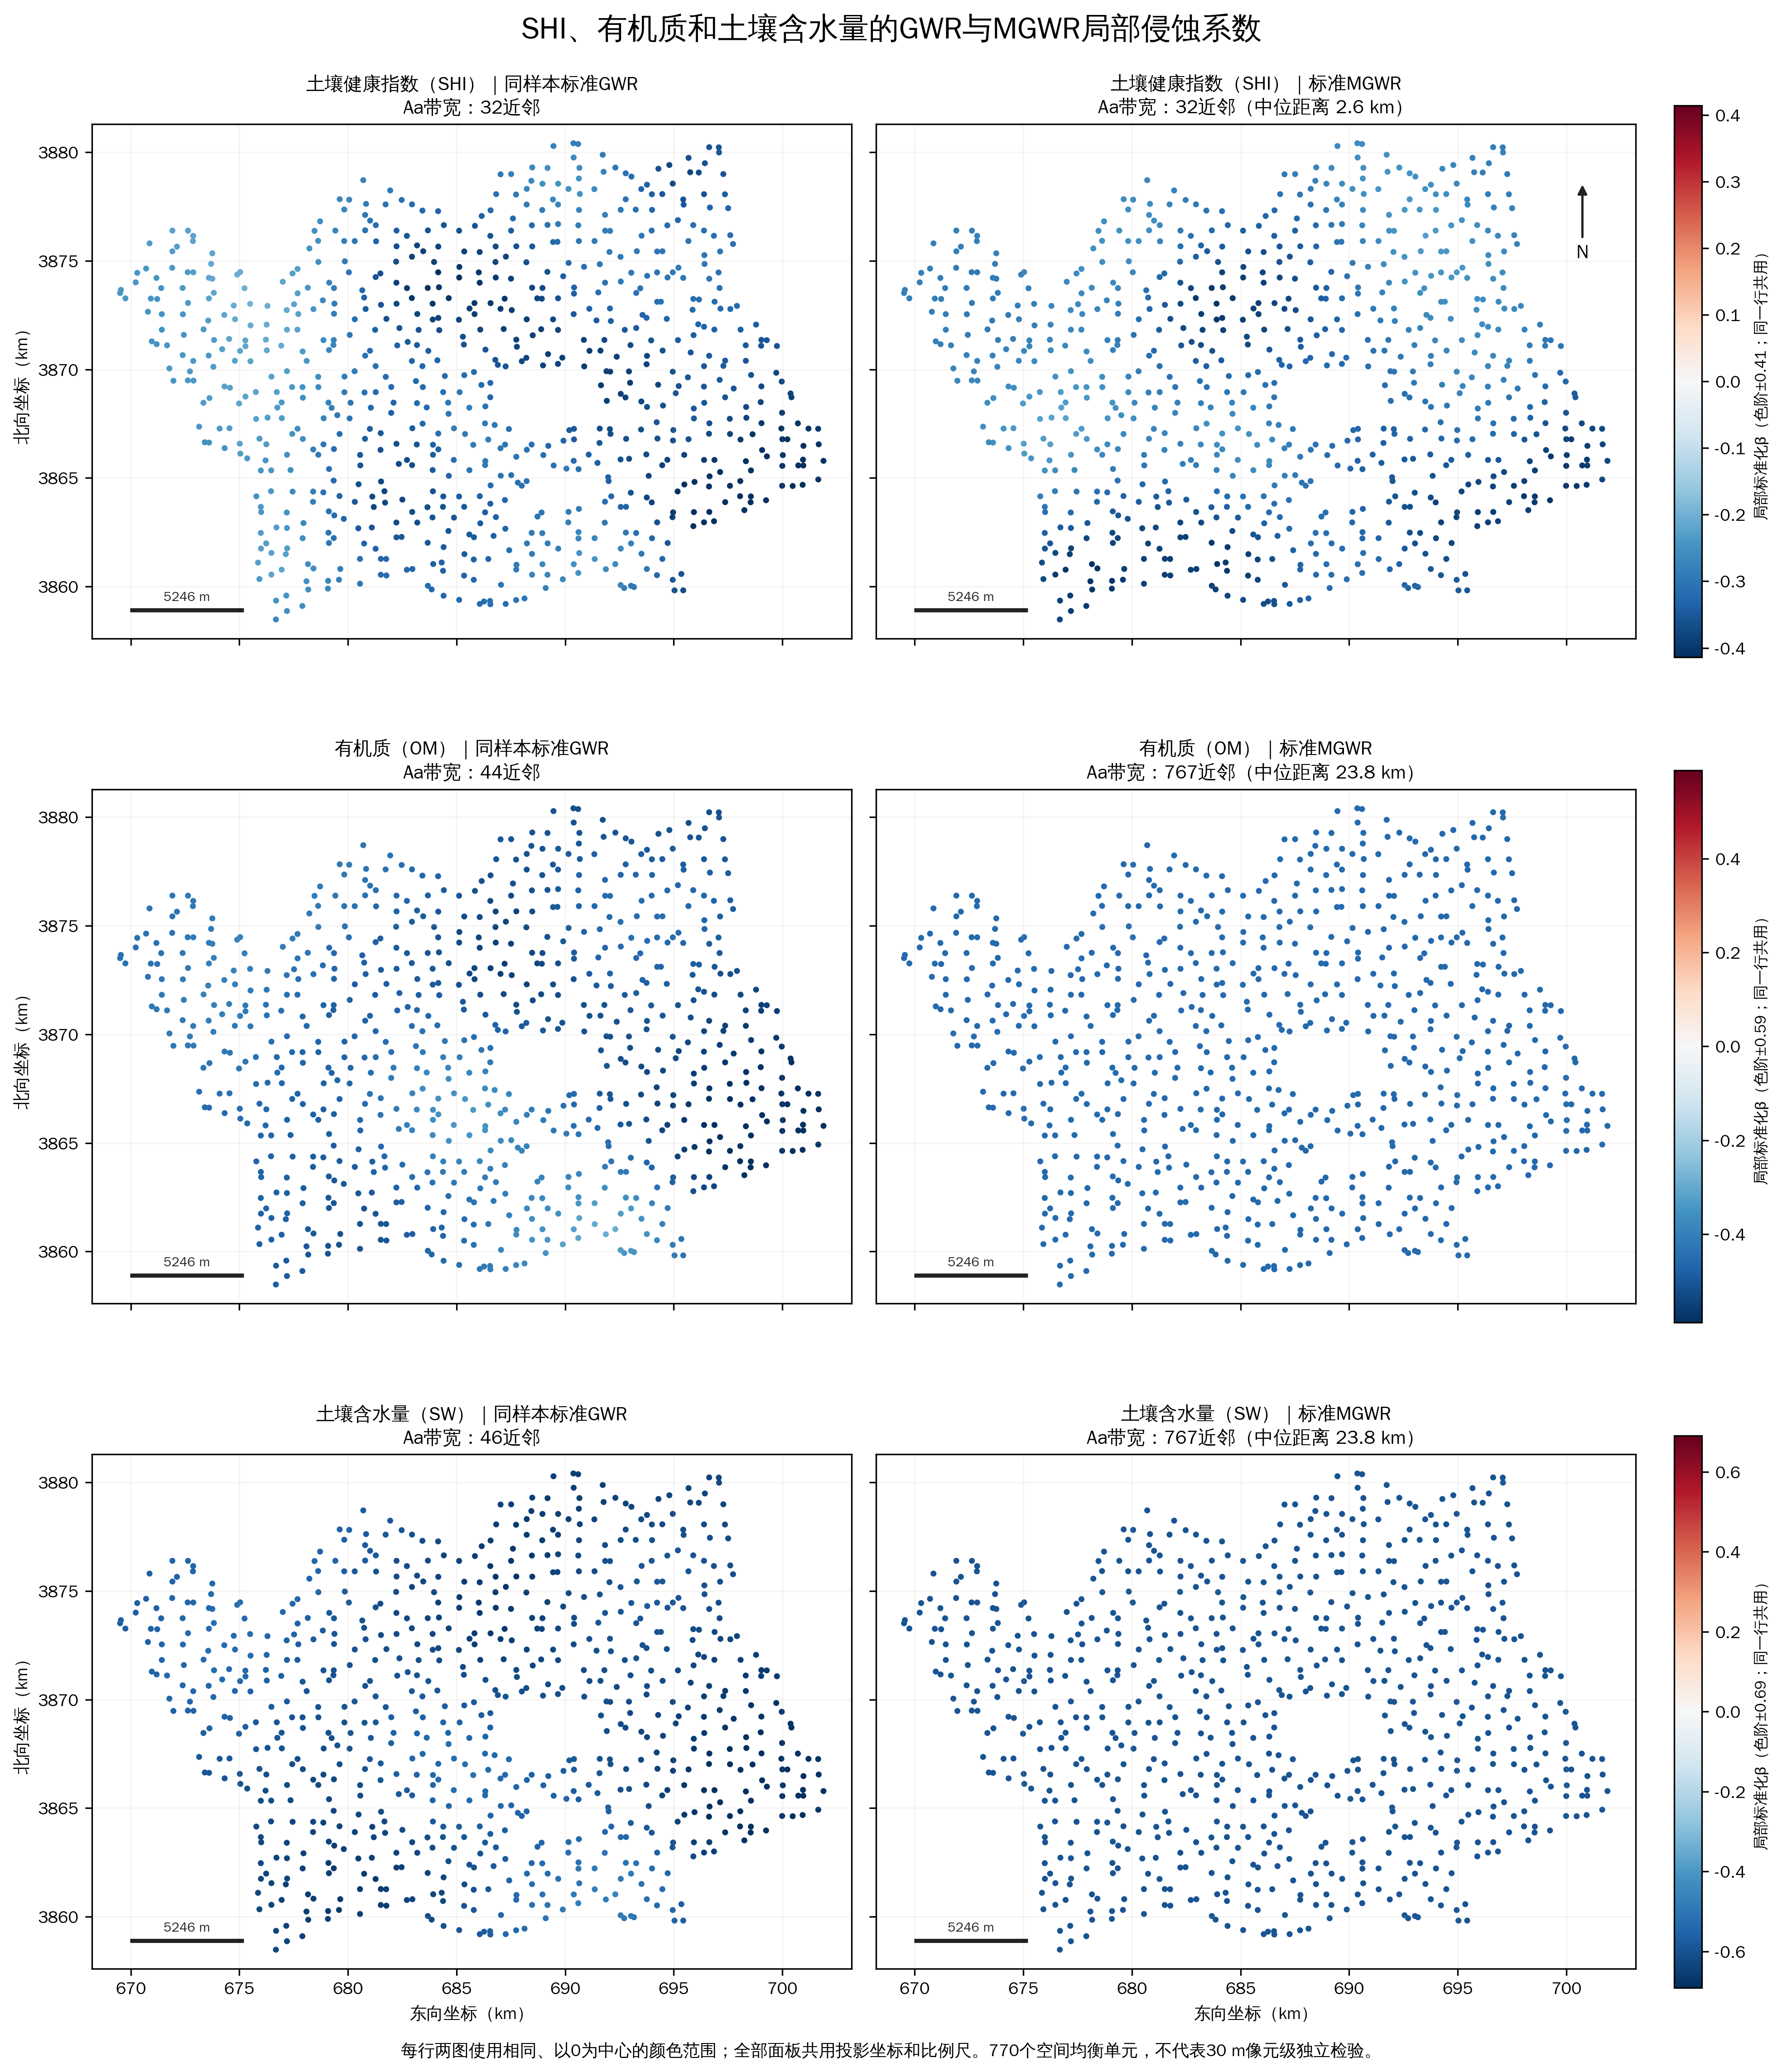
\includegraphics{reviews/2026-11-02/phase-j/figures/B_gwr_mgwr_spatial_patterns.png}
\caption{SHI、OM、SW 在共同空间位置上的 GWR 和 MGWR
系数图。每个局部估计显示该位置附近的关联模式，不代表该地的因果效应。}
\end{figure}

I-5还测试局地随机森林、SHAP、ALE 和空间变化系数 GAM。SHAP
可以粗略理解为把模型的预测变化分摊给不同变量；ALE
则画出变量变化和预测值之间的局部平均关系。SHI、OM、SW 的局地随机森林 R²
中位数约为0.610、0.618、0.736，但随机切分会让相邻点同时进入训练和验证，不能当作空间独立测试。它们解释的是预测模型如何工作，不是侵蚀的因果作用。空间块测试中，空间变化系数
GAM 相对全局 GAM 的 R² 增益仅约SHI +0.014、OM +0.007、SW
+0.005，说明更复杂的空间曲面只带来很小的额外预测信息。

I-6用100近邻局部相关和八邻接双变量 LISA
描述邻域聚集，并进行999次置换和多重比较调整。LISA
可理解为检查``这个格子和它附近的格子是否形成一块相似或相反的区域''。同位高侵蚀-低
SHI
的单元为2,473个（约33.5\%）；这和``本格侵蚀高、邻居的健康低''的邻域类别不是同一个统计概念。GWR
与收缩模型给出的负向热点数量分别可为2,484和3,124个单元，说明热点范围会随局部模型而变。

\begin{figure}
\centering
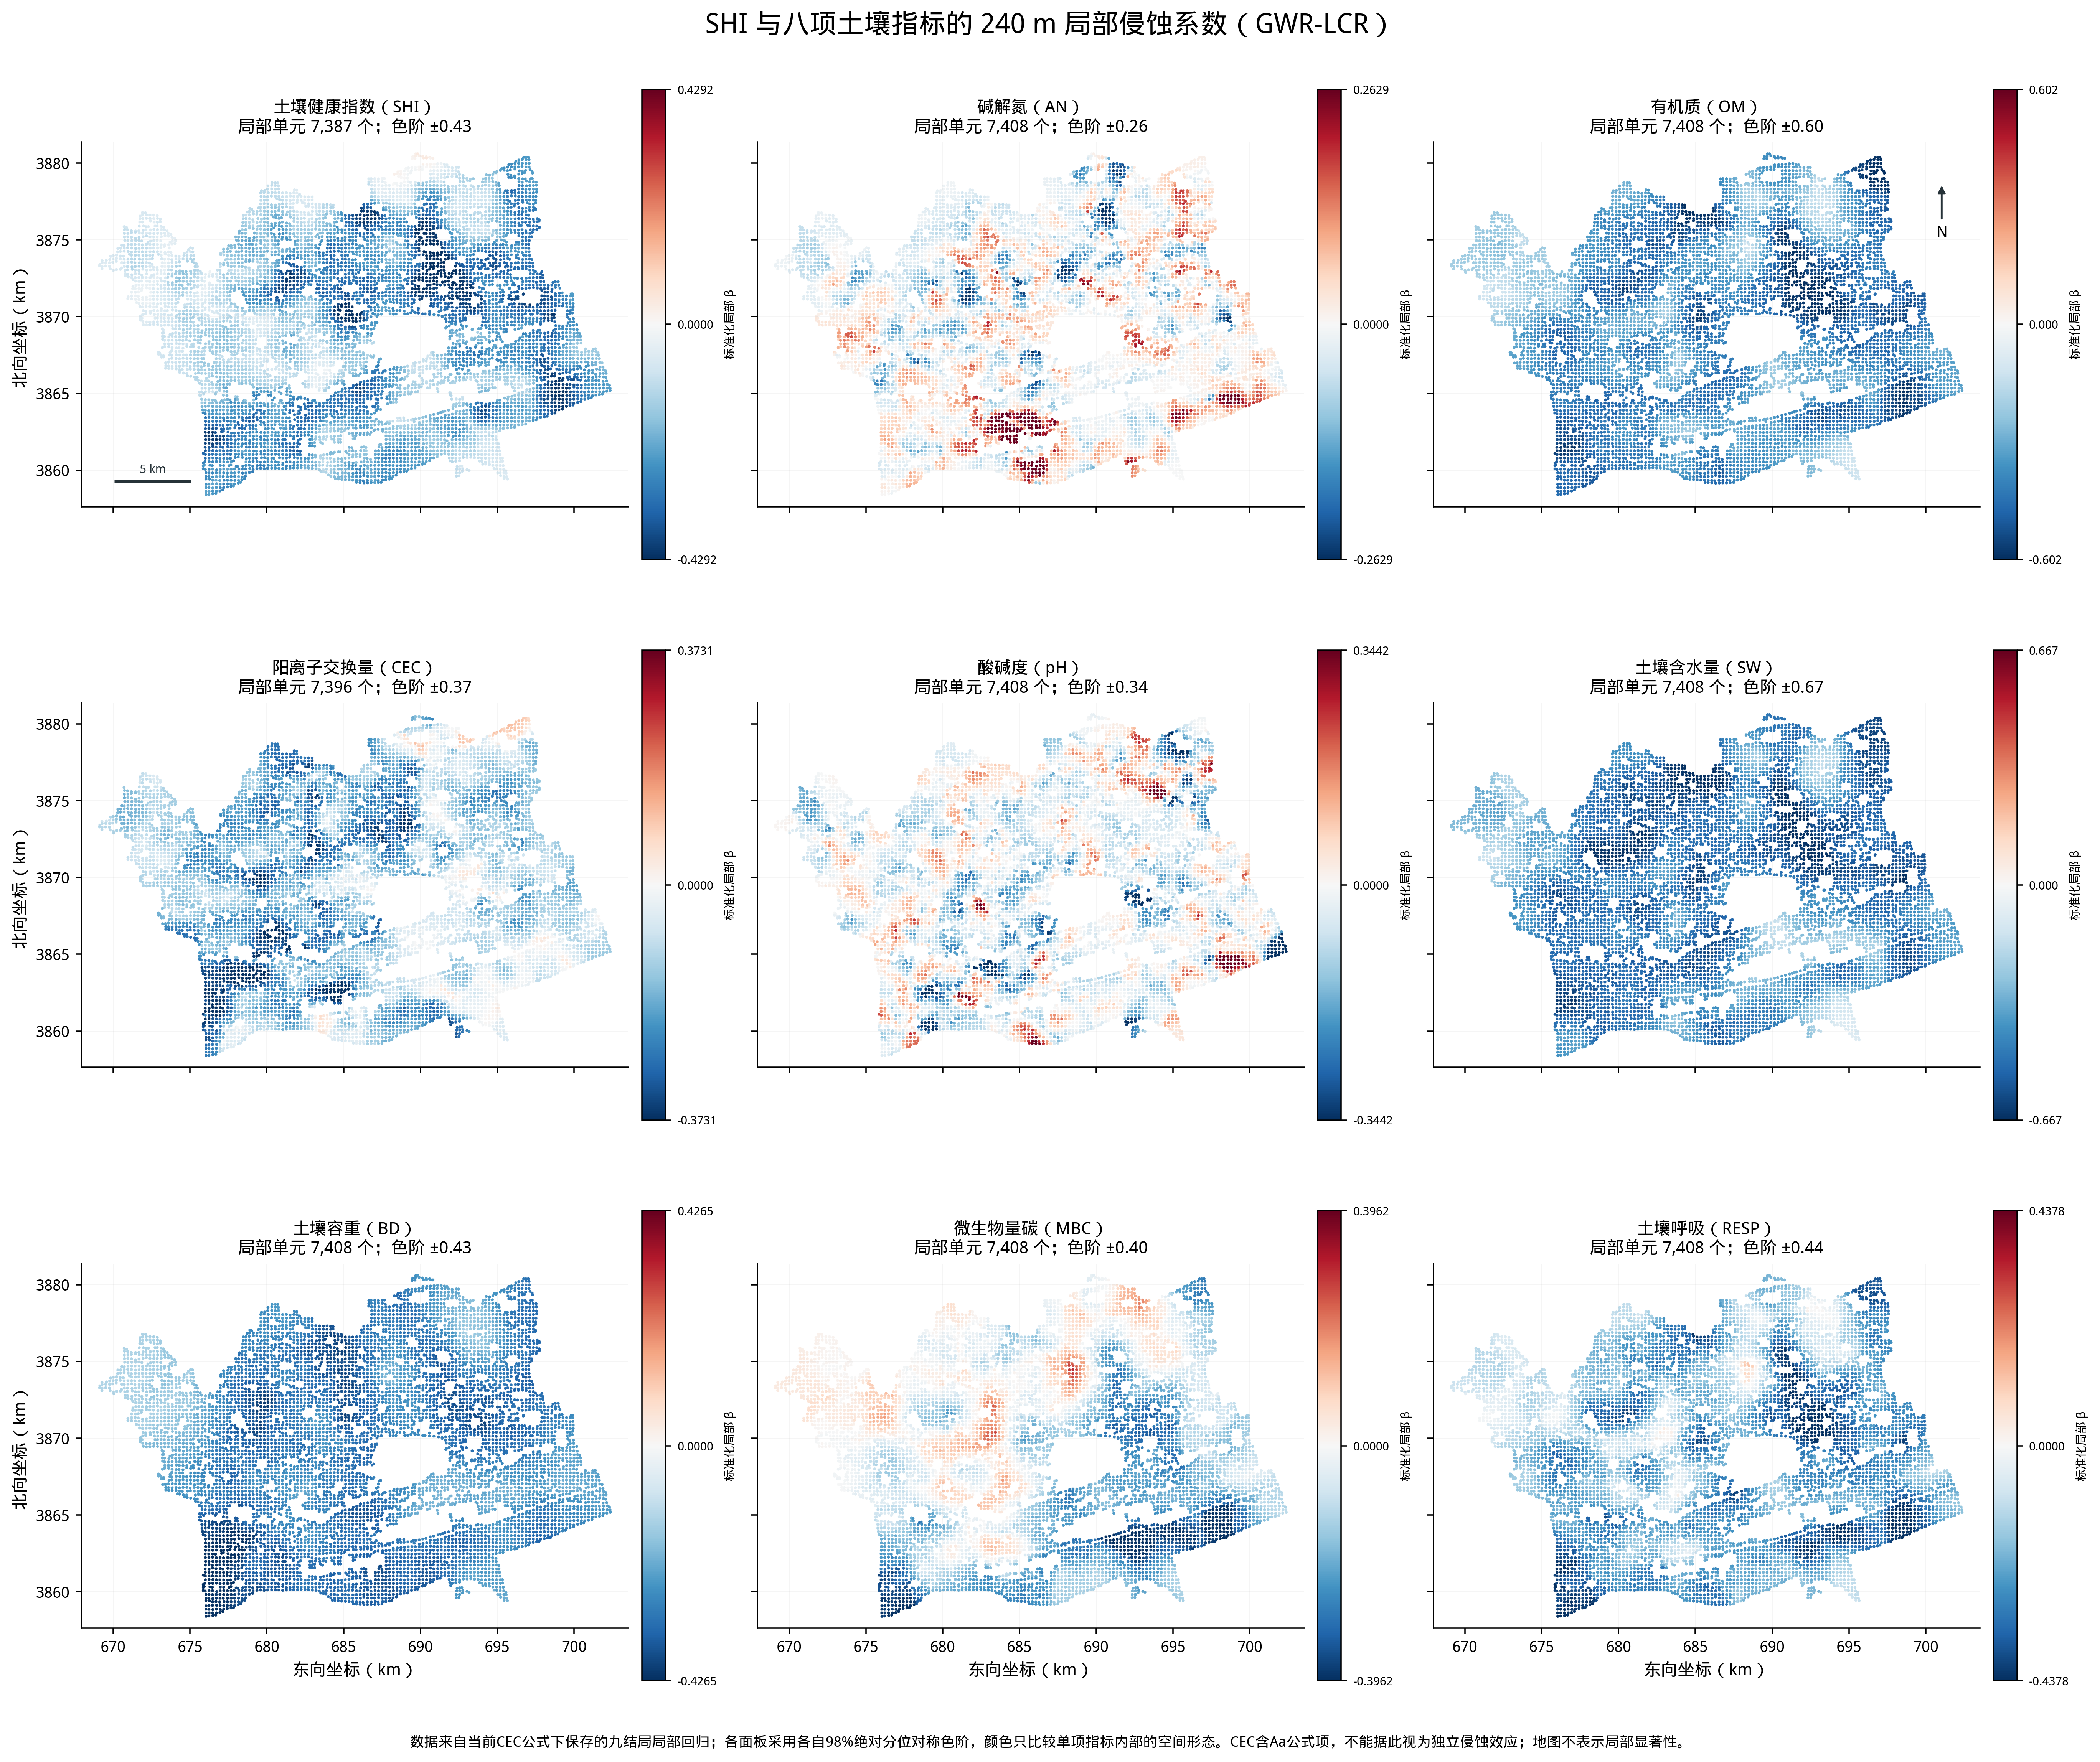
\includegraphics{reviews/2026-11-02/phase-j/figures/supplementary/U_nine_outcome_local_beta_maps.png}
\caption{九项健康结果的局部系数图。地图显示不同地区估计的方向与大小；局部系数不是田间试验得出的因果效应。}
\end{figure}

\hypertarget{cec-ux6570ux636eux6062ux590dux4e3aux4ec0ux4e48ux8fd9ux4e00ux6b65ux4f1aux6539ux53d8ux89e3ux91ca}{%
\subsection{5.6 CEC
数据恢复：为什么这一步会改变解释？}\label{cec-ux6570ux636eux6062ux590dux4e3aux4ec0ux4e48ux8fd9ux4e00ux6b65ux4f1aux6539ux53d8ux89e3ux91ca}}

项目中途发现，过去给出的 CEC
图层经过人为添加了与侵蚀有关的正向关系。用户找到了恢复原始数值的公式，并确认两个最大值来自两张完整对齐栅格的全域有效像元。项目按最终公式恢复
CEC，并把恢复后的数值作为项目当前的 CEC 使用：

\textbf{CEC = (原 CEC - 20 × (Aa\_20yr / 143.00503540039062 + Aa\_2020 /
48.76557540893555)) / 2.9 + 18}

这里143.00503540039062是 Aa\_20yr 全域最大值；48.76557540893555是
Aa\_2020 全域最大值。按公式逐像元复算后，有效 CEC
为387,448格，范围约16.725814到26.836542，与保存的当前 CEC
最大绝对差为0。

所有当前图表把该指标标成``CEC''，不写``校正CEC''。此前使用旧数值的图另行归档，不放进当前图集中；重复图已清理。当前
Phase J
图表也使用这套数值。公式、范围和逐像元核对记录见\href{reviews/2026-10-31/phase-i/cec-correction/CEC_CORRECTION_REANALYSIS.md}{CEC
数据恢复重分析}。

但公式里直接减去了两期侵蚀值，所以当前 CEC
与侵蚀的负向关联有一部分是公式结构直接带进去的。比如两张图即便没有新的生态过程证据，只要按公式计算，也会产生特定方向的数值关系。因此
CEC
结果可以用于当前项目数据的一致分析，却不能单独作为``侵蚀导致土壤化学性质变化''的独立验证。这一点会在所有
CEC 结论中保留。

\hypertarget{phase-jux628aux591aux79cdux7ed3ux679cux5408ux5728ux4e00ux8d77ux5e76ux753bux8defux5f84ux56fe}{%
\subsection{5.7 Phase
J：把多种结果合在一起，并画路径图}\label{phase-jux628aux591aux79cdux7ed3ux679cux5408ux5728ux4e00ux8d77ux5e76ux753bux8defux5f84ux56fe}}

Phase J 的 r10
综合运行使用两张各392,527行的对齐输入表。按模型所需环境变量筛选后，核心完整案例为293,145格；240米汇总有7,387个单元和293,633个支撑像元。这里的``支撑像元''是用于形成240米平均值的30米格子数，不是额外的独立测量。最新运行状态和检查数字见\href{reviews/2026-11-02/phase-j/RUN_STATUS.md}{Phase
J 运行记录}。

Phase J
将已有全域相关、配对、局部空间结果、路径回归和图件整合。它还运行了多类路径模型：记录中共有1,582条成功拟合状态，但``软件显示运行成功''只说明计算结束，不说明每个模型都适合做科学推断。不同模型的标准误和拟合指标假设不同，尤其是相邻像元有空间依赖时，普通模型可能把不确定性估得过小。

为了让``SEM路径图''容易理解，可以把它看作一张假设关系的箭头图：箭头表示模型在其他变量给定时估计到的条件关联，不是自动证明``前一个变量造成后一个变量''。Phase
J 比较了几种结构：

\begin{longtable}[]{@{}ll@{}}
\toprule
路径结构 & 箭头大意 \\
\midrule
\endhead
S1 & 侵蚀 → 物理、化学、生物活动三个指标组 \\
S2 & 侵蚀 → 三个指标组；三组再与 SHI 相连；同时保留侵蚀 → SHI \\
S3 & 与 S2 类似，但不保留侵蚀 → SHI 的直接箭头 \\
S4 & 侵蚀 → 物理 → 化学 → 生物活动 → SHI 的链式假设 \\
S5 & 侵蚀分别指向九项健康结果 \\
S6 & 把``是否为正侵蚀''和``正侵蚀有多大''拆成两条信息 \\
\bottomrule
\end{longtable}

这些都是待比较的统计结构，不是已由实验确认的生物学因果链。物理、化学、生物综合值使用了简化的指标组合；没有足够来源核实每项的方向和权重，因此不能说它们是验证过的``潜在健康因子''。

模型对环境背景的控制也分层比较：M0不加入环境控制；M1加入高程、TWI、NDVI、LST和土壤类型；M2用环境变量的主成分摘要加土类；M3在M1基础上再加入空间坐标。主成分可以理解为把许多相近的环境变量压缩成少数几个综合刻度。模型控制越多不一定越``正确''，要看它是否符合研究问题、输入质量和空间检验。

在核心环境控制模型 M1
中，侵蚀与物理、化学、生物活动综合值的标准化条件系数约为
-0.389、-0.251、-0.066。保留侵蚀到 SHI 直接路径的候选模型里，直接系数约
-0.113，R²约0.601；加入侵蚀后 R²
增量约0.0079。通俗地说：在这个具体模型中，侵蚀与综合指数仍有负向条件关联，但它让
SHI 预测解释度增加不到1个百分点。

加入空间坐标的 M3 表观 R²约0.651；不加环境控制的 M0 中，侵蚀带来的
R²增量约0.017。不能按这些数字挑``最正确的模型''：坐标可能只是帮助模型画出平滑空间图纹，不加环境控制又容易混入共同变化。它们回答的是不同模型条件下的预测/关联问题，均不能作因果贡献排名。

结构方程软件 lavaan 的常规 ML
拟合指标没有自动修正空间依赖；自由度为0的模型无法用 CFI、TLI、RMSEA
判断结构是否合适。项目内 Mode-B PLS 路径没有 bootstrap
区间和空间稳健推断。因此 Phase J
的路径图是模型探索图，不能独立确认``侵蚀通过某指标传导导致健康变化''。

\begin{figure}
\centering
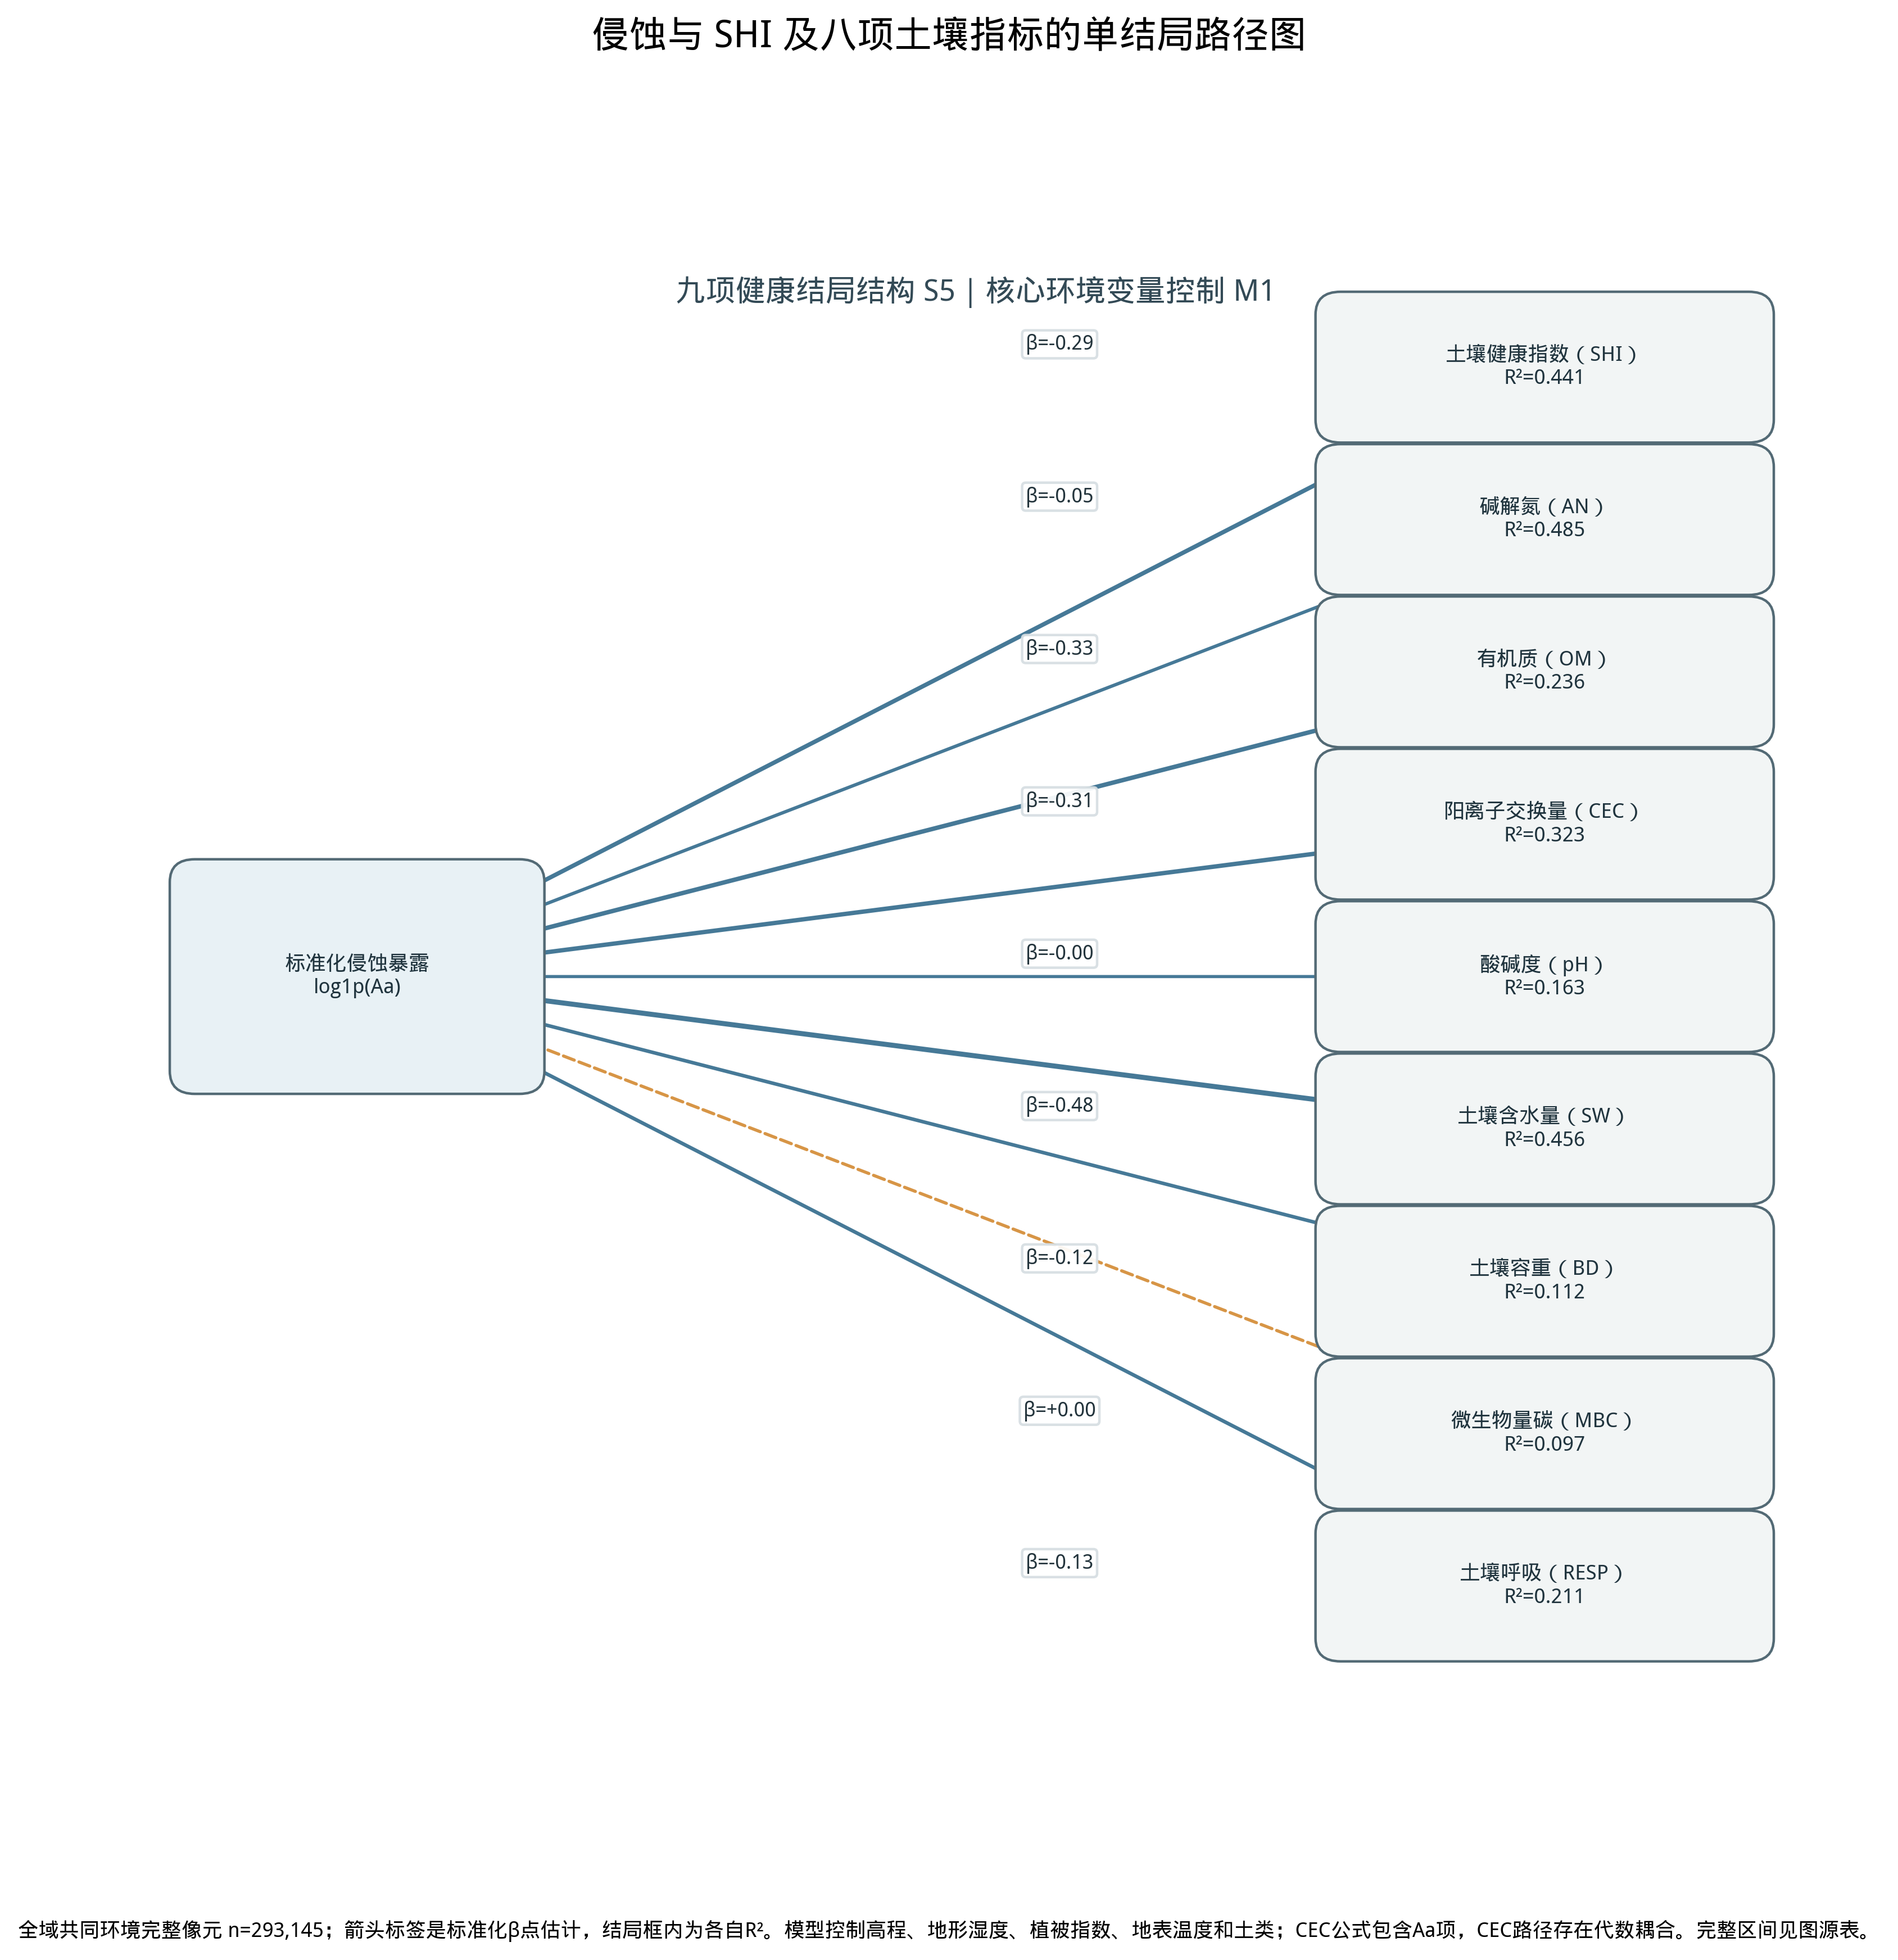
\includegraphics{reviews/2026-11-02/phase-j/figures/supplementary/Y_sem_nine_outcome_diagram.png}
\caption{九项健康结果的路径结构示意。箭头和系数来自探索性模型，图中的
R²是模型内拟合描述，不是因果证明。}
\end{figure}

Phase J 还根据一份本地章节草稿尝试重建 SHI
的指标方向和评分。重建结果与当前正式使用的 SHI
地图仅相关0.730，RMSE为0.118，平均偏差为+0.105；CEC在99.998\%的像元落到上限评分。这表示草稿规则没有复现当前
SHI 制图，不能拿它替换现有图或据此重估路径和 GWR。项目保留既有
SHI，并把这次重建只作为敏感性检查。要真正核实
SHI，还需找到原始方向、隶属函数、权重和制图脚本。Phase J
综合报告对模型结构和结果边界有更完整说明，见\href{reviews/2026-11-02/phase-j/reports/PHASE_J_ACADEMIC_RESEARCH_REPORT.md}{Phase
J 学术报告}。

\hypertarget{i-8ux628aux7ed3ux679cux753bux6210ux5019ux9009ux7a7aux95f4ux533a}{%
\subsection{5.8
I-8：把结果画成候选空间区}\label{i-8ux628aux7ed3ux679cux753bux6210ux5019ux9009ux7a7aux95f4ux533a}}

I-8把30米图汇总成约240米单元，在7,387个完整空间单元上组合 Aa、SHI 和 SHI
局部 GWR 系数。分区使用 Aa
的80\%分位、局部系数的20\%分位、Aa中位数和SHI低分位等 Oracle
阈值。分位数就是把样本按大小排序后取某个位置；它适合描述当前样本，不自动等于政策标准。

\begin{longtable}[]{@{}lrr@{}}
\toprule
候选区 & 单元数 / 面积等价 & Aa 均值 / SHI 均值 / 局部斜率中位数 \\
\midrule
\endhead
T1：高 Aa、强负向响应 & 623 / 约18.88 km² & 15.670 / 0.549 / -0.567 \\
T2：高 Aa、较弱负向响应 & 842 / 约24.00 km² & 14.951 / 0.584 / -0.327 \\
T3：低 Aa、低 SHI & 60 / 约2.05 km² & 5.480 / 0.562 / -0.368 \\
T4：环境敏感候选 & 961 / 约38.77 km² & 5.109 / 0.628 / -0.311 \\
其他或未分类 & 4,901 / 约180.57 km² & 5.324 / 0.624 / -0.301 \\
\bottomrule
\end{longtable}

表中依次列出 Aa 均值、SHI 均值和局部斜率中位数。T1
是最适合优先实地核查的探索候选；T2 可检查环境和农艺因素是否提供缓冲；T3
的低 SHI 不一定由侵蚀解释，可先查土壤状况；T4
用来提出环境敏感地点的后续问题；其他地区未落入上述探索分类。

面积是按共同完整案例中实际纳入的30米支撑像元换算的``面积等价''，不应把240米方格都假定为完整有效覆盖。T1是后续现场检查的候选，不是已验证的治理风险区；所有分位阈值也不是法定界线。

\begin{figure}
\centering
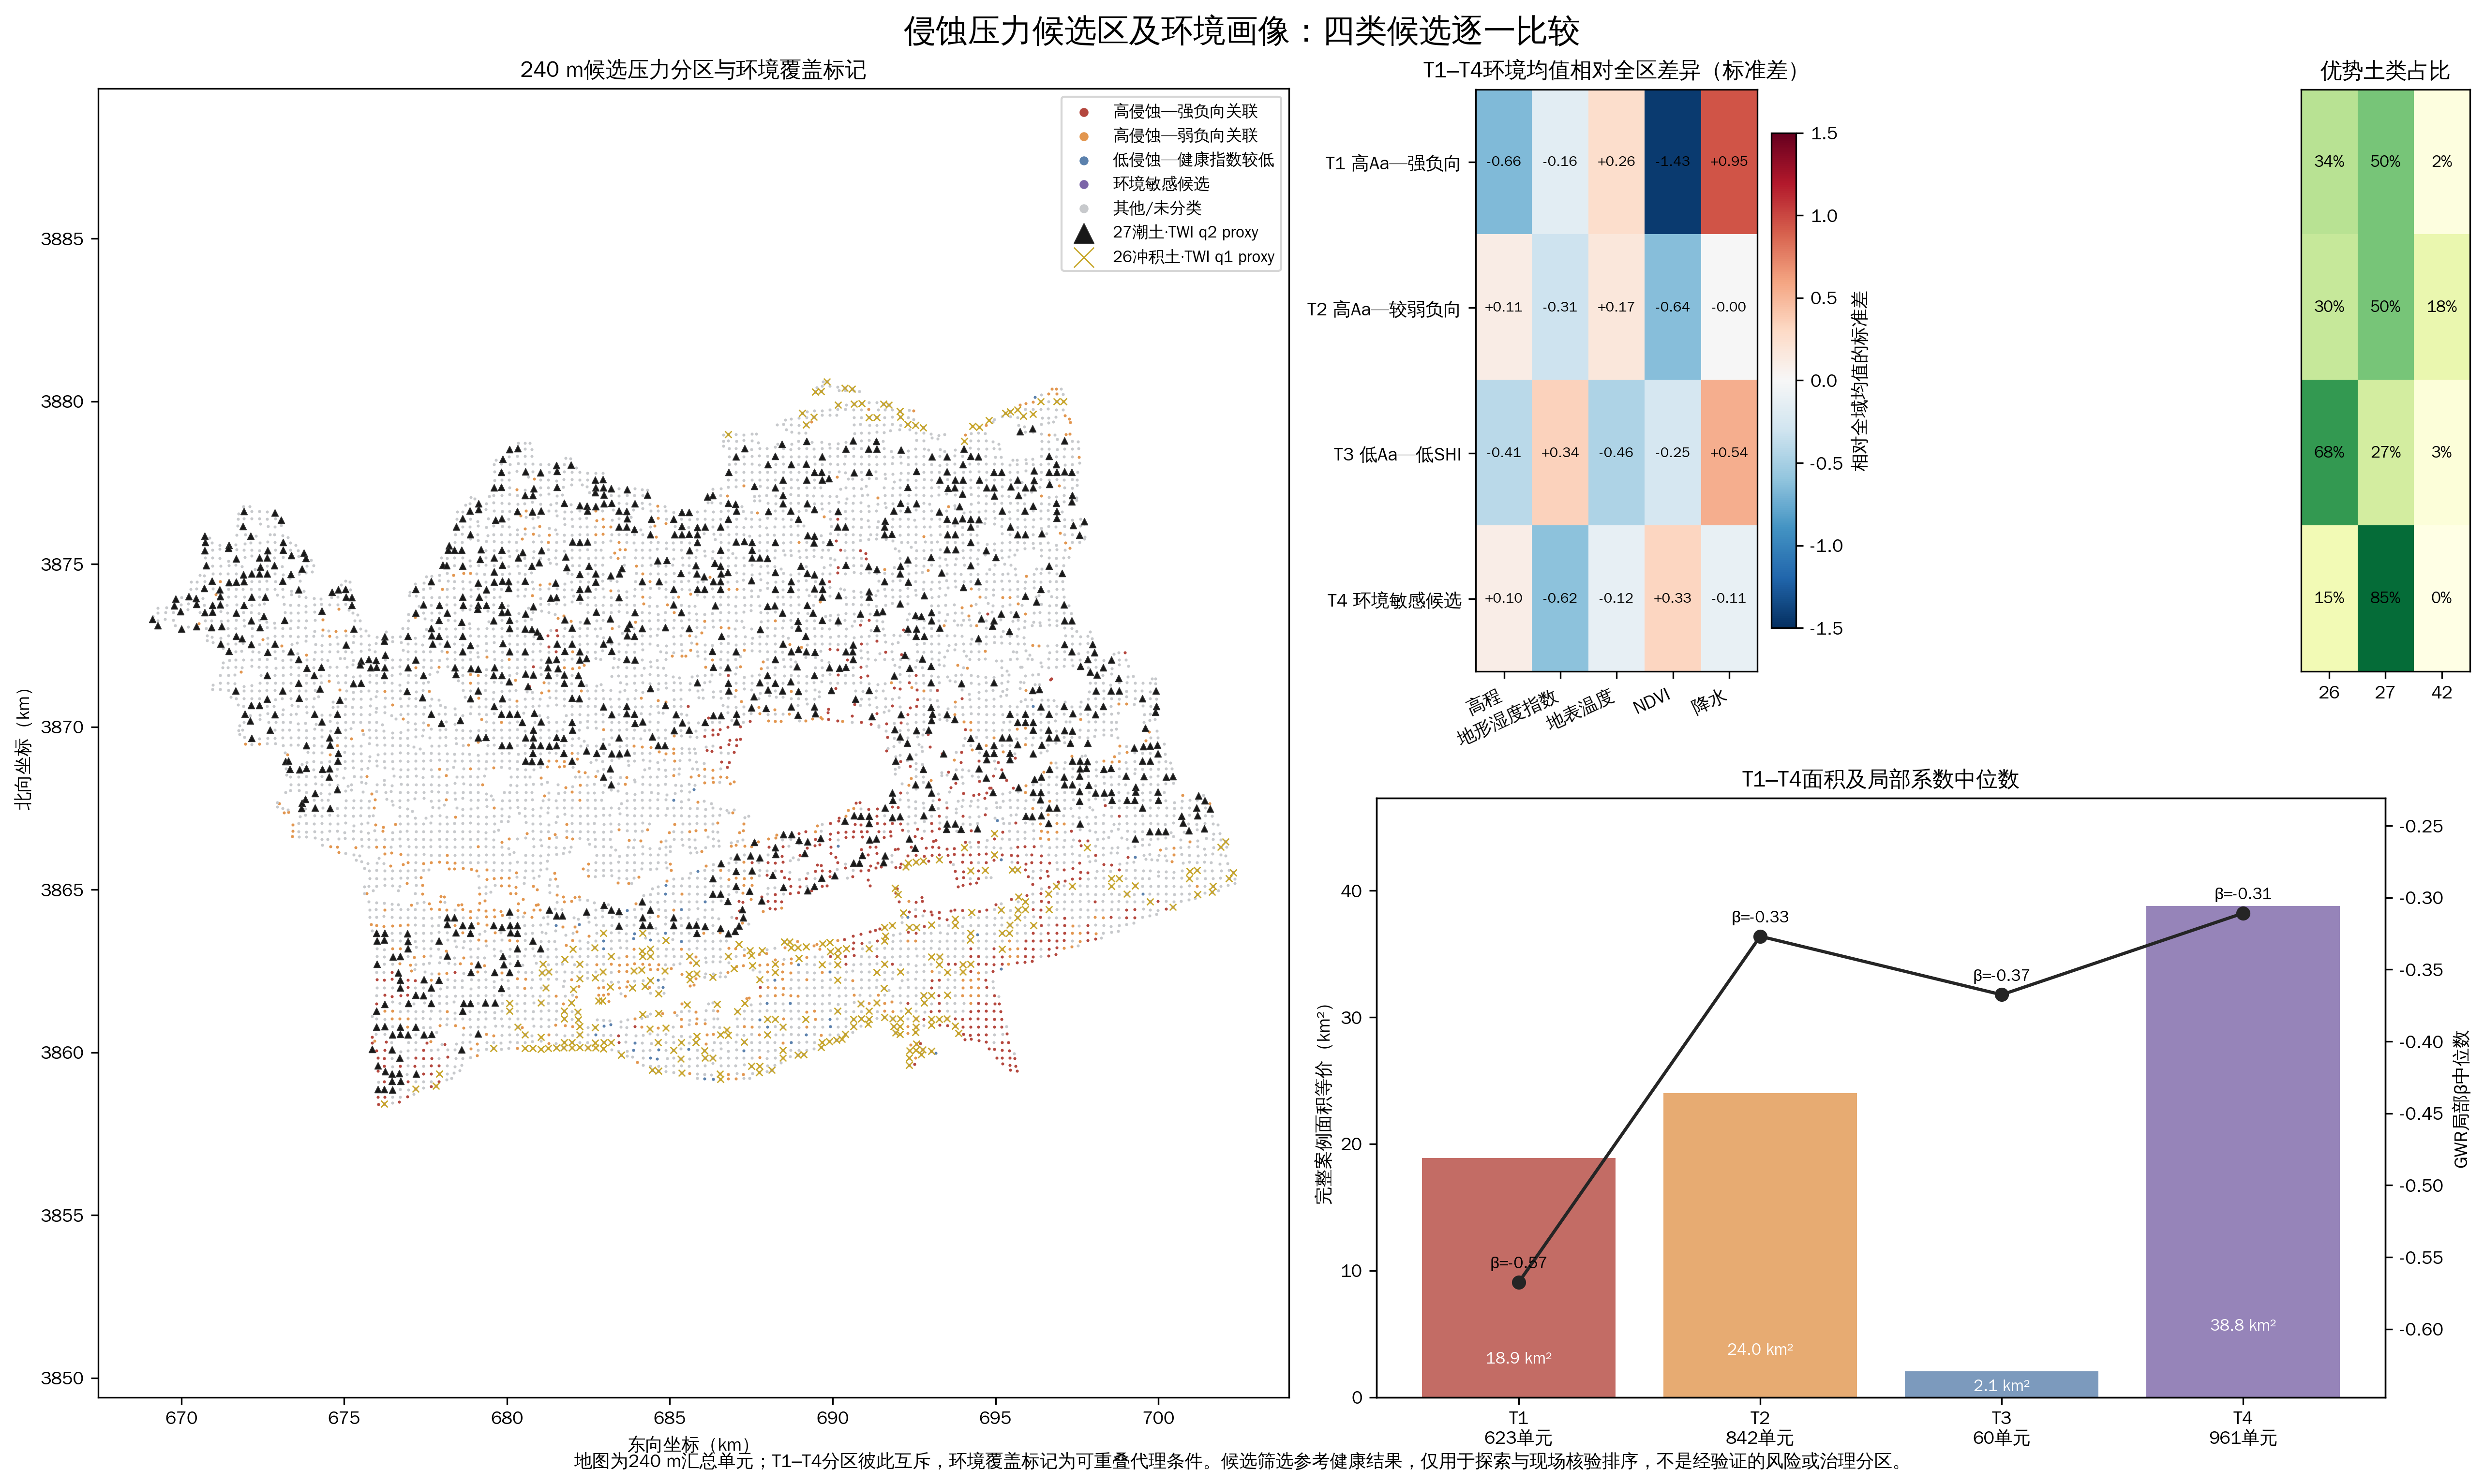
\includegraphics{reviews/2026-11-02/phase-j/figures/C_stress_sensitive_environment_zones.png}
\caption{探索性空间分区图。T1-T4由样本分位点和局部系数组合得到，适合安排核查，不等于正式风险地图。}
\end{figure}

\hypertarget{ux516dux56feux96c6ux548cux6210ux679cux6574ux7406ux505aux4e86ux4ec0ux4e48}{%
\section{六、图集和成果整理做了什么？}\label{ux516dux56feux96c6ux548cux6210ux679cux6574ux7406ux505aux4e86ux4ec0ux4e48}}

项目先后发现过中文字体显示不完整、重复图、CEC
旧版本图、图名难懂、图集漏掉后续 GWR/空间图等问题。因此当前成果整理时：

\begin{enumerate}
\def\labelenumi{\arabic{enumi}.}
\tightlist
\item
  将当前图表中的指标名统一写为``CEC''，并确认当前图表使用恢复后的数值。
\item
  将旧 CEC 图另行归档，不放入当前图集。
\item
  检查并删除图集中重复图卡，保留中文字体显示正常的版本。
\item
  补入九项指标局部 GWR、SHI/SW/OM 重点空间图、候选分区，以及多种 SEM
  路径结构图。
\item
  给图增加中文题名和尽量通俗的解释，标明地图像元、空间单元、模型系数和候选阈值的含义。
\end{enumerate}

Phase J 图册有 A-Z
共26幅图，覆盖总体关联、匹配、GWR/MGWR、局部空间图和路径结构；最新项目总图集状态记录170张去重图卡，将不同阶段的产出收在一起，并对重复图和旧
CEC
图做了筛除。完整入口见\href{FIGURE_ATLAS.html}{项目总图集}。正式长报告和图集是互补的：报告讲逻辑，图集方便逐图查看。

\hypertarget{ux4e03ux628aux76eeux524dux7ed3ux679cux8bb2ux6210ux6700ux6734ux7d20ux7684ux8bdd}{%
\section{七、把目前结果讲成最朴素的话}\label{ux4e03ux628aux76eeux524dux7ed3ux679cux8bb2ux6210ux6700ux6734ux7d20ux7684ux8bdd}}

\begin{enumerate}
\def\labelenumi{\arabic{enumi}.}
\tightlist
\item
  在这张预测地图上，侵蚀较高的格子往往也有较低的 SW、SHI 和 OM 数值。
\item
  把一些环境较相近、侵蚀不同的地点配对后，这三个指标的差值关系仍多为负，但弱一些。
\item
  这种关系在地图不同地方并不完全一样；局部回归和空间聚集图能提供线索，但不同方法画出的范围会变。
\item
  SHI、SW、OM适合作为本阶段重点讲解对象：SW在全域数值关联最强，SHI代表综合结果，OM代表与其方向较一致的化学指标。这里说的是``重点关联''，不是已经证明的三种因果效应。
\item
  CEC 的当前负相关部分由恢复公式直接带入，不能拿它单独证明侵蚀影响了
  CEC。
\item
  路径图说明若干可供进一步检验的关系结构，不是现实世界因果箭头已经被实验确认。
\item
  T1 等空间区是排序和现场核验的候选区，不是已经确认的治理红线。
\item
  所以最稳妥的总结是：项目找到了值得继续核验的空间关联线索，但正式设计和独立验证尚未完成。
\end{enumerate}

\hypertarget{ux516bux73b0ux5728ux8fd8ux4e0dux80fdux56deux7b54ux4ec0ux4e48ux4e0bux4e00ux6b65ux7f3aux4ec0ux4e48}{%
\section{八、现在还不能回答什么？下一步缺什么？}\label{ux516bux73b0ux5728ux8fd8ux4e0dux80fdux56deux7b54ux4ec0ux4e48ux4e0bux4e00ux6b65ux7f3aux4ec0ux4e48}}

\hypertarget{ux6570ux636eux6765ux6e90ux4e0eux6b63ux5f0fux9636ux6bb5}{%
\subsection{8.1
数据来源与正式阶段}\label{ux6570ux636eux6765ux6e90ux4e0eux6b63ux5f0fux9636ux6bb5}}

\begin{itemize}
\tightlist
\item
  \textbf{Aa 单位和时间口径：}
  文件名支持``20年平均''和``2020年''的区分，但单位、精确年份跨度和制图来源还需要正式元数据或原始说明。
\item
  \textbf{研究区面积差异：}
  掩膜面积约353.274平方公里，既有研究记载约347.877平方公里；矢量边界配套文件缺失，无法独立解释差值。
\item
  \textbf{环境变量完整核查：}
  变量年份、原始分辨率、与随机森林和侵蚀制图共享的输入信息，需要正式整理并锁定。
\item
  \textbf{正式匹配设计：} 当前 Oracle
  中许多选择依赖健康结果；它们不能直接搬去正式模式充当预设设计。
\item
  \textbf{正式响应阶段：} G4 未锁定前，Oracle 的相关、GWR、SEM
  不能算正式 G5 通过。
\end{itemize}

\hypertarget{ux7ed3ux679cux6765ux6e90ux4e0eux72ecux7acbux6027}{%
\subsection{8.2
结果来源与独立性}\label{ux7ed3ux679cux6765ux6e90ux4e0eux72ecux7acbux6027}}

\begin{itemize}
\tightlist
\item
  \textbf{像元不是独立样点。}
  相邻地图格子相似；空间块能减少部分泄漏，但不能把预测图变成独立实测。
\item
  \textbf{预测图不是现场测量。} SHI
  和八项指标沿用随机森林预测面；图层误差、训练点分布和共享环境变量都会影响关联。
\item
  \textbf{变量可能共享制图信息。}
  如果侵蚀图和健康图用过共同地形或遥感信息，即使两者有关系，也可能有共同来源。
\item
  \textbf{Oracle 结果经过搜索。}
  试了很多模型和分组后再挑最强结果，会使表观关系偏大；应优先报告未筛选基线和空间外推表现。
\item
  \textbf{CEC 有公式耦合。} 其当前公式显式含有两期
  Aa，方向相关不能独立说明生态机制。
\item
  \textbf{SHI 公式尚待追源。} 当前沿用既有 SHI；候选草稿没有成功复现它。
\item
  \textbf{PCNM 对照未完成。} 项目历史上已有 PCNM
  分析，应保留；但本轮找不到可读结果表，不能说两种方法一致或谁更强。
\item
  \textbf{路径图不等于因果模型。}
  复合指标权重、方向来源和空间稳健不确定性仍不足；模型成功运行也不替代科学验证。
\item
  \textbf{外部现场验证尚未提供。} T1-T4
  需要与现场调查、田块和管理信息核对后，才能讨论实际治理含义。
\end{itemize}

\hypertarget{ux8fd9ux6761ux7814ux7a76ux4e3bux7ebfux600eux6837ux7ee7ux7eed}{%
\subsection{8.3
这条研究主线怎样继续}\label{ux8fd9ux6761ux7814ux7a76ux4e3bux7ebfux600eux6837ux7ee7ux7eed}}

若要从探索线索走向正式结论，最优先的工作是补齐侵蚀图单位、年份和来源说明，解决研究区边界面积差异，核实环境变量来源与年份，确定不看健康结果的正式匹配设计，再按阶段门开展健康响应和空间推断。之后找到既有
PCNM 结果表及 SHI 制图公式，与新的结果逐项对照；最后再对 T1
候选区做现场核验。每一步都应记录配置、样本单位、排除规则和未通过的检查。

这些是从现有缺口自然推导出的后续步骤，不表示本报告已经完成它们。正式研究继续按\href{WORKFLOW.md}{工作流程}、\href{RESEARCH_PLAN.md}{研究方案}、\href{DATA_REQUIREMENTS.md}{数据要求}推进。

\hypertarget{ux4e5dux4e13ux4e1aux8bcdux6c47ux5c0fux8bcdux5178}{%
\section{九、专业词汇小词典}\label{ux4e5dux4e13ux4e1aux8bcdux6c47ux5c0fux8bcdux5178}}

\begin{itemize}
\tightlist
\item
  \textbf{栅格、像元：} 地图上的一个小方格；本项目每格约30米见方。
\item
  \textbf{掩膜：} 一张``只留下研究区域''的模板；模板外的格子不参加统计。
\item
  \textbf{对齐：} 让不同透明方格纸上的小格边界和位置重合。
\item
  \textbf{NoData：} 这个格子没有可用数字，不能当成0。
\item
  \textbf{环境匹配：}
  给环境相近的两个地点配成一组，再比较侵蚀不同的一端。
\item
  \textbf{标准化：} 把不同单位的数值改成相同刻度，便于比较大小。
\item
  \textbf{相关：} 两件事的数值是否常一起升降；它本身不说明谁造成谁。
\item
  \textbf{Spearman 相关：} 先看名次，再看两组名次是否一起变化；范围 -1
  到 +1。
\item
  \textbf{OLS 普通线性回归：}
  用一条直线概括输入和结果之间的平均变化；需要额外处理空间相邻带来的依赖。
\item
  \textbf{回归系数：}
  在指定模型中，输入增加时结果平均怎样变化；要结合单位和控制条件看。
\item
  \textbf{R²：}
  模型在这批数据上能跟随数值变化到什么程度；不等于因果，也不保证换地区仍然有效。
\item
  \textbf{空间块验证：}
  把一整片地留出来检验，避免把训练格子旁边的近邻放进测试集。
\item
  \textbf{GWR：}
  给地图不同位置分别估计附近的关系，观察关系是否有地方差异。
\item
  \textbf{GWR-LCR：}
  在局部回归里给不稳定系数加限制，减少相似变量导致的剧烈波动。
\item
  \textbf{MGWR：} 允许不同输入各自用不同大小的地图邻域来估计。
\item
  \textbf{LISA：}
  检查一个格子和周围格子是否一起形成高值、低值或相反的聚集。
\item
  \textbf{热点：}
  某种指标在地图上聚集较多的一片区域；热点取决于指标和算法。
\item
  \textbf{GAM：} 允许曲线弯曲的回归模型，不强迫关系只能是一条直线。
\item
  \textbf{SEM 路径图：} 把模型设定的关联画成箭头；箭头不是因果证明。
\item
  \textbf{PCNM：}
  一种用空间位置构造控制变量的方法；本项目保留既有结果，但还缺本轮可读的对照表。
\item
  \textbf{Oracle 探索：}
  获准尝试多种分组和模型以寻找线索；筛选结果需要单独披露，不能冒充正式验证。
\end{itemize}

\hypertarget{ux5341ux4e3bux8981ux8d44ux6599ux5165ux53e3}{%
\section{十、主要资料入口}\label{ux5341ux4e3bux8981ux8d44ux6599ux5165ux53e3}}

\begin{itemize}
\tightlist
\item
  \href{RESEARCH_CHARTER.md}{研究总纲}：项目研究问题与长期边界。
\item
  \href{governance/RESEARCH_STAGE_GATES.md}{研究阶段门}：正式研究何时可以进入下一步。
\item
  \href{RESEARCH_PLAN.md}{研究方案}、\href{METHODOLOGY.md}{方法说明}、\href{DATA_REQUIREMENTS.md}{数据要求}和\href{WORKFLOW.md}{工作流程}：项目的具体执行办法。
\item
  \href{DEVELOPMENT_LOG.md}{开发日志}与\href{DECISIONS.md}{决策记录}：项目过程、参数选择和限制的时间线。
\item
  \href{reviews/2026-10-26/PHASE_F_RESEARCH_REPORT.md}{Phase F
  报告}、\href{reviews/2026-10-27/phase-g/PHASE_G_RESEARCH_REPORT.md}{Phase
  G
  报告}、\href{reviews/2026-10-28/phase-h/PHASE_H_EXPLORATORY_REPORT.md}{Phase
  H
  报告}和\href{reviews/2026-10-29/phase-h/LOW_EROSION_REGIME_RESEARCH_REPORT.md}{低侵蚀专题}：早期探索记录。
\item
  \href{reviews/2026-10-31/phase-i/PHASE_I_FINAL_RESEARCH_REPORT.md}{Phase
  I
  综合结果}与\href{reviews/2026-10-31/phase-i/PHASE_I_CLOSURE_REPORT.md}{Phase
  I 结题说明}：全域、匹配、异质性、空间和分区结果。
\item
  \href{reviews/2026-11-02/phase-j/reports/PHASE_J_ACADEMIC_RESEARCH_REPORT.md}{Phase
  J 学术报告}和\href{reviews/2026-11-02/phase-j/RUN_STATUS.md}{Phase J
  当前运行状态}：综合路径分析、最新图件与数据状态。
\item
  \href{reviews/2026-10-31/phase-i/cec-correction/CEC_CORRECTION_REANALYSIS.md}{CEC
  数据恢复重分析}：公式、有效像元和范围核对。
\item
  \href{FIGURE_ATLAS.html}{项目总图集}：跨阶段图表入口。
\end{itemize}

\end{document}
